\chapter{Numbers, Functions, and Models}
\label{chap:numbers-functions-models}

The first chapter began with motion and ended with a promise:

\[
\text{make the input close enough, and the output becomes as close as required.}
\]

For \(s(t)=t^2\), the average velocity from \(t=2\) to \(t=2+h\) was

\[
\frac{s(2+h)-s(2)}{h}=4+h,
\qquad h\neq 0.
\]

The error from the expected value \(4\) was

\[
|(4+h)-4|=|h|.
\]

That small calculation already contains the next need. Calculus needs a way to speak about closeness, intervals around a point, and errors that can be made as small as we want.

The real line is the measuring tape.

\section{The real line and intervals}
\label{sec:real-line-intervals}

Numbers do two jobs for us. They locate points, and they measure distances between points. The same number \(3\) can mean a position on a line, a length, a time, a temperature, or an error bound. Calculus depends on moving between these meanings without confusion.

\subsection{Points as numbers}
\label{subsec:points-as-numbers}

We picture the real numbers on a horizontal line. Positive numbers lie to the right of \(0\). Negative numbers lie to the left.

\begin{figure}[h]
\centering
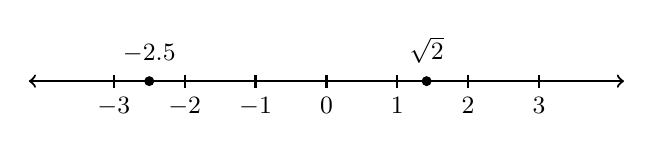
\begin{tikzpicture}[scale=0.9, every node/.style={font=\small}]
  \draw[<->, thick] (-4.2,0) -- (4.2,0);
  \foreach \x in {-3,-2,-1,0,1,2,3} {
    \draw[thick] (\x,0.09) -- (\x,-0.09);
    \node[below] at (\x,-0.09) {\(\x\)};
  }
  \fill (1.414,0) circle (2pt);
  \node[above] at (1.414,0.12) {\(\sqrt2\)};
  \fill (-2.5,0) circle (2pt);
  \node[above] at (-2.5,0.12) {\(-2.5\)};
\end{tikzpicture}
\caption{The real line turns numbers into points and distances.}
\label{fig:real-line-basic}
\end{figure}

When we write

\[
a<b,
\]

we mean that \(a\) lies to the left of \(b\) on the real line. Equivalently, \(b-a\) is positive.

When we write

\[
a\le b,
\]

we mean that \(a<b\) or \(a=b\).

\paragraph{Example.}
The inequality

\[
1.99<2<2.01
\]

says that \(2\) lies between \(1.99\) and \(2.01\). It also says that \(2\) is within \(0.01\) of both endpoints.

This is already the kind of statement calculus will use. A limiting process often traps a number inside smaller and smaller intervals.

\subsection{Open, closed, and half-open intervals}
\label{subsec:intervals}

An \emph{interval} is an unbroken piece of the real line. If two numbers are in the interval, then every number between them is also in the interval.

For \(a<b\), we use the following notation:

\[
(a,b)=\{x\in\mathbb R: a<x<b\},
\]

\[
[a,b]=\{x\in\mathbb R: a\le x\le b\},
\]

\[
(a,b]=\{x\in\mathbb R: a<x\le b\},
\]

\[
[a,b)=\{x\in\mathbb R: a\le x<b\}.
\]

The parentheses mean that an endpoint is not included. The square bracket means that an endpoint is included.

\begin{figure}[h]
\centering
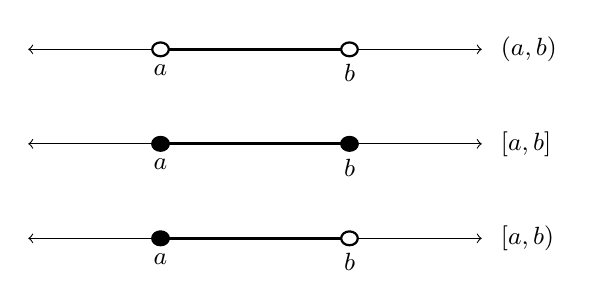
\begin{tikzpicture}[xscale=1.2, every node/.style={font=\small}]
  % open interval
  \draw[<->] (-0.4,2.4) -- (4.4,2.4);
  \draw[very thick] (1,2.4) -- (3,2.4);
  \draw[fill=white, thick] (1,2.4) circle (2.5pt);
  \draw[fill=white, thick] (3,2.4) circle (2.5pt);
  \node[below] at (1,2.33) {\(a\)};
  \node[below] at (3,2.33) {\(b\)};
  \node[right] at (4.5,2.4) {\((a,b)\)};

  % closed interval
  \draw[<->] (-0.4,1.2) -- (4.4,1.2);
  \draw[very thick] (1,1.2) -- (3,1.2);
  \draw[fill=black, thick] (1,1.2) circle (2.5pt);
  \draw[fill=black, thick] (3,1.2) circle (2.5pt);
  \node[below] at (1,1.13) {\(a\)};
  \node[below] at (3,1.13) {\(b\)};
  \node[right] at (4.5,1.2) {\([a,b]\)};

  % half-open interval
  \draw[<->] (-0.4,0) -- (4.4,0);
  \draw[very thick] (1,0) -- (3,0);
  \draw[fill=black, thick] (1,0) circle (2.5pt);
  \draw[fill=white, thick] (3,0) circle (2.5pt);
  \node[below] at (1,-0.07) {\(a\)};
  \node[below] at (3,-0.07) {\(b\)};
  \node[right] at (4.5,0) {\([a,b)\)};
\end{tikzpicture}
\caption{Open circles mean endpoints are excluded. Filled circles mean endpoints are included.}
\label{fig:interval-types}
\end{figure}

There are also infinite intervals:

\[
(a,\infty)=\{x\in\mathbb R:x>a\},
\]

\[
(-\infty,b]=\{x\in\mathbb R:x\le b\}.
\]

The symbols \(\infty\) and \(-\infty\) are not real numbers. They are directions. So we never write a square bracket next to \(\infty\).

\paragraph{Example.}
The set of all times from \(0\) to \(3\) hours, including both endpoints, is

\[
[0,3].
\]

The set of all positive times is

\[
(0,\infty).
\]

The set of all nonnegative times is

\[
[0,\infty).
\]

\paragraph{A punctured interval.}
Limits often look near a point without using the point itself. The set

\[
(a-\varepsilon,a+\varepsilon)\setminus\{a\}
\]

is called a \emph{punctured interval} around \(a\). It contains numbers close to \(a\), but not \(a\) itself.

This is exactly what happened in the average velocity

\[
\frac{s(2+h)-s(2)}{h}.
\]

We wanted \(h\) close to \(0\), but \(h=0\) was not allowed because the denominator would be \(0\).

\subsection{Absolute value as distance}
\label{subsec:absolute-value-distance}

The absolute value of a number measures its distance from \(0\):

\[
|x|=
\begin{cases}
x, & x\ge 0,\\
-x, & x<0.
\end{cases}
\]

Thus

\[
|3|=3,
\qquad
|-3|=3,
\qquad
|0|=0.
\]

Distance is never negative.

The distance between two numbers \(x\) and \(a\) is

\[
|x-a|.
\]

It does not matter which number is written first, because

\[
|x-a|=|a-x|.
\]

\begin{figure}[h]
\centering
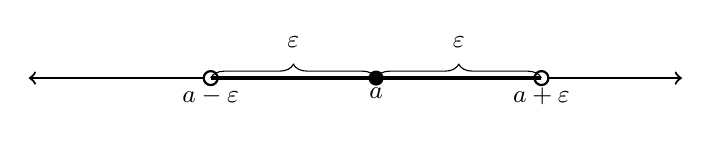
\begin{tikzpicture}[scale=1.05, every node/.style={font=\small}]
  \draw[<->, thick] (-0.7,0) -- (7.2,0);

  \coordinate (L) at (1.5,0);
  \coordinate (A) at (3.5,0);
  \coordinate (R) at (5.5,0);

  \draw[fill=black] (A) circle (2.4pt);
  \draw[fill=white, thick] (L) circle (2.4pt);
  \draw[fill=white, thick] (R) circle (2.4pt);

  \node[below] at (L) {\(a-\varepsilon\)};
  \node[below] at (A) {\(a\)};
  \node[below] at (R) {\(a+\varepsilon\)};

  \draw[decorate, decoration={brace, amplitude=5pt}] (L) -- (A);
  \node[above] at (2.5,0.25) {\(\varepsilon\)};

  \draw[decorate, decoration={brace, amplitude=5pt}] (A) -- (R);
  \node[above] at (4.5,0.25) {\(\varepsilon\)};

  \draw[very thick] (L) -- (R);
\end{tikzpicture}
\caption{The inequality \(|x-a|<\varepsilon\) means that \(x\) lies within distance \(\varepsilon\) of \(a\).}
\label{fig:absolute-value-neighborhood}
\end{figure}

The most useful translation is this one:

\[
\boxed{|x-a|<\varepsilon
\quad \Longleftrightarrow \quad
a-\varepsilon<x<a+\varepsilon,}
\qquad \varepsilon>0.
\]

In words: \(x\) is within \(\varepsilon\) of \(a\) exactly when \(x\) lies between \(a-\varepsilon\) and \(a+\varepsilon\).

\paragraph{Proof.}
The inequality

\[
|x-a|<\varepsilon
\]

means that the distance from \(x\) to \(a\) is less than \(\varepsilon\). On the line, this says that \(x\) cannot be \(\varepsilon\) or more units to the left of \(a\), and cannot be \(\varepsilon\) or more units to the right of \(a\). Therefore

\[
a-\varepsilon<x<a+\varepsilon.
\]

Algebraically, the same statement is

\[
-\varepsilon<x-a<\varepsilon.
\]

Adding \(a\) to all three parts gives

\[
a-\varepsilon<x<a+\varepsilon.
\]

The steps reverse, so the two statements are equivalent.

\paragraph{Example.}
Solve

\[
|x-5|<\frac12.
\]

This means that \(x\) is within \(\frac12\) of \(5\). Therefore

\[
5-\frac12<x<5+\frac12,
\]

so

\[
\frac92<x<\frac{11}{2}.
\]

In interval notation,

\[
x\in\left(\frac92,\frac{11}{2}\right).
\]

If the inequality were

\[
|x-5|\le \frac12,
\]

the answer would be the closed interval

\[
\left[\frac92,\frac{11}{2}\right].
\]

\paragraph{Why \(\varepsilon>0\) appears.}
The number \(\varepsilon\) is usually an allowed error. Allowed errors must be positive.

If \(\varepsilon=0\), then

\[
|x-a|<0
\]

has no solution, because a distance cannot be negative.

If \(\varepsilon<0\), the inequality

\[
|x-a|<\varepsilon
\]

also has no solution.

So whenever we write \(|x-a|<\varepsilon\) to describe closeness, we mean \(\varepsilon>0\).

\subsection{Inequalities as a way to control error}
\label{subsec:inequalities-control-error}

The word \emph{error} does not mean a mistake. It means the difference between a quantity and the value we want.

If an approximation \(A\) is meant to approximate a true value \(T\), then the absolute error is

\[
|A-T|.
\]

For example, using \(3.14\) to approximate \(\pi\) gives absolute error

\[
|\pi-3.14|.
\]

When we say

\[
|\pi-3.14|<0.002,
\]

we are saying that \(3.14\) is within \(0.002\) of \(\pi\).

Calculus uses inequalities to force errors to become small.

\paragraph{Example: controlling the average velocity error.}
For \(s(t)=t^2\), the average velocity from \(t=2\) to \(t=2+h\) is

\[
\frac{s(2+h)-s(2)}{h}=4+h,
\qquad h\neq 0.
\]

The error from \(4\) is

\[
|(4+h)-4|=|h|.
\]

If we want this error to be less than \(0.01\), it is enough to require

\[
0<|h|<0.01.
\]

The condition \(h\neq 0\) is written as \(0<|h|\). The condition that \(h\) is close to \(0\) is written as \(|h|<0.01\).

\paragraph{Example: a slightly less obvious error.}
For \(s(t)=t^3\), the average velocity from \(t=2\) to \(t=2+h\) is

\[
\frac{s(2+h)-s(2)}{h}
=
\frac{(2+h)^3-8}{h}.
\]

For \(h\neq 0\),

\[
\frac{(2+h)^3-8}{h}
=
\frac{8+12h+6h^2+h^3-8}{h}
=
12+6h+h^2.
\]

The number we expect as \(h\) gets close to \(0\) is \(12\). The error is

\[
|(12+6h+h^2)-12|
=
|6h+h^2|.
\]

This is not exactly \(|h|\), but we can control it by \(|h|\). If \(|h|<1\), then

\[
|6h+h^2|
\le 6|h|+|h|^2
<6|h|+|h|
=
7|h|.
\]

So to make the error less than \(0.01\), it is enough to require

\[
7|h|<0.01,
\]

or

\[
|h|<\frac{0.01}{7}.
\]

This is the basic shape of a limit proof. We do not merely say that the numbers seem to approach \(12\). We show how to make the error smaller than any chosen tolerance.

\begin{quote}
\textbf{The language of control.}
An inequality such as

\[
|A-T|<\varepsilon
\]

means that the approximation \(A\) is within the allowed error \(\varepsilon\) of the target value \(T\).
\end{quote}

The real line now gives us a way to talk about closeness. But there is a deeper question hiding under the picture. Is the line really unbroken? Are there numbers for all the points that geometry asks for?

The answer is yes for the real numbers. It is no for the rational numbers. That difference is one reason calculus is built on \(\mathbb R\), not just on fractions.

\section{Completeness and the idea of no gaps}
\label{sec:completeness-no-gaps}

The last section used the real line as if every point on it had a number. That is a stronger promise than it may first appear.

Fractions are already very rich. Between any two fractions there is another fraction. For example, between \(1.41\) and \(1.42\) lies

\[
1.415=\frac{1415}{1000}.
\]

Still, fractions alone leave gaps. Geometry finds one of those gaps in a unit square.

\begin{quote}
\textbf{First-reading note.}
This section explains why the real numbers, not only rational numbers, are the right setting for calculus. You may read the proof details lightly on a first pass. The main idea is simple: calculus needs an unbroken number line because limits can point to numbers that no finite decimal or fraction exactly equals.
\end{quote}

\subsection{Rational numbers and the missing square root}
\label{subsec:rational-missing-sqrt}

Draw a square whose sides have length \(1\). Its diagonal has length \(d\). By the Pythagorean theorem,

\[
d^2=1^2+1^2=2.
\]

So the diagonal length should be a number whose square is \(2\). We call it \(\sqrt2\).

\begin{figure}[h]
\centering
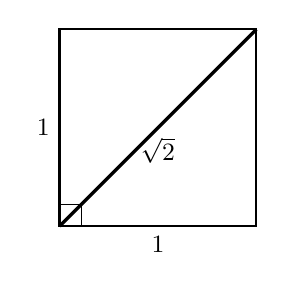
\begin{tikzpicture}[scale=1.25, every node/.style={font=\small}]
  \draw[thick] (0,0) rectangle (2,2);
  \draw[very thick] (0,0) -- (2,2);
  \node[left] at (0,1) {\(1\)};
  \node[below] at (1,0) {\(1\)};
  \node[below] at (1,1) {\(\sqrt2\)};
  \draw (0.22,0) -- (0.22,0.22) -- (0,0.22);
\end{tikzpicture}
\caption{The diagonal of a unit square has length \(\sqrt2\), the number whose square is \(2\).}
\label{fig:unit-square-sqrt2}
\end{figure}

Decimal approximations quickly trap this number:

\[
1.4^2=1.96<2,
\qquad
1.5^2=2.25>2,
\]

so

\[
1.4<\sqrt2<1.5.
\]

A sharper trap is

\[
1.41^2=1.9881<2,
\qquad
1.42^2=2.0164>2,
\]

so

\[
1.41<\sqrt2<1.42.
\]

Sharper still,

\[
1.414^2=1.999396<2,
\qquad
1.415^2=2.002225>2,
\]

so

\[
1.414<\sqrt2<1.415.
\]

All these decimals are rational numbers. But the number they are closing in on is not rational.

\paragraph{Optional proof that \(\sqrt2\) is not rational.}
Suppose, for contradiction, that

\[
\sqrt2=\frac{p}{q},
\]

where \(p\) and \(q\) are integers with no common factor and \(q\neq 0\). Squaring both sides gives

\[
2=\frac{p^2}{q^2},
\]

so

\[
p^2=2q^2.
\]

Thus \(p^2\) is even. Therefore \(p\) is even. Write

\[
p=2k.
\]

Then

\[
p^2=4k^2.
\]

Substitute into \(p^2=2q^2\):

\[
4k^2=2q^2,
\]

so

\[
q^2=2k^2.
\]

Thus \(q^2\) is even, so \(q\) is even.

We have shown that both \(p\) and \(q\) are even. That contradicts the assumption that \(p\) and \(q\) had no common factor.

Therefore \(\sqrt2\) is not rational.

\begin{quote}
\textbf{Moral.}
Fractions can approximate the diagonal of a unit square as closely as we want, but no fraction equals it.
\end{quote}

This is the first warning that ``many numbers'' is not the same as ``no gaps.''

\subsection{Nested intervals}
\label{subsec:nested-intervals}

The decimal approximations to \(\sqrt2\) give a sequence of smaller and smaller intervals:

\[
[1.4,1.5],
\]

\[
[1.41,1.42],
\]

\[
[1.414,1.415],
\]

and so on. Each interval contains the next, and the lengths shrink:

\[
0.1,\quad 0.01,\quad 0.001,\quad \ldots
\]

\begin{figure}[h]
\centering
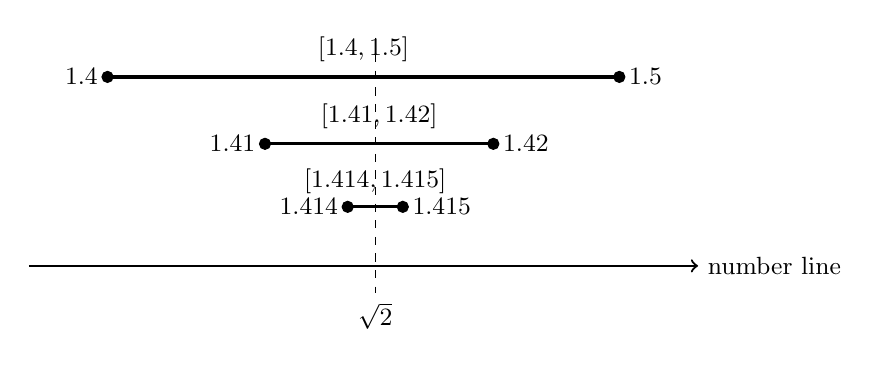
\begin{tikzpicture}[every node/.style={font=\small}]
  \draw[->, thick] (0,0) -- (8.5,0);
  \node[right] at (8.5,0) {number line};

  \draw[dashed] (4.4,2.9) -- (4.4,-0.35);
  \node[below] at (4.4,-0.35) {\(\sqrt2\)};

  \draw[very thick] (1.0,2.4) -- (7.5,2.4);
  \draw[fill=black] (1.0,2.4) circle (2pt);
  \draw[fill=black] (7.5,2.4) circle (2pt);
  \node[left] at (1.0,2.4) {\(1.4\)};
  \node[right] at (7.5,2.4) {\(1.5\)};
  \node at (4.25,2.75) {\([1.4,1.5]\)};

  \draw[very thick] (3.0,1.55) -- (5.9,1.55);
  \draw[fill=black] (3.0,1.55) circle (2pt);
  \draw[fill=black] (5.9,1.55) circle (2pt);
  \node[left] at (3.0,1.55) {\(1.41\)};
  \node[right] at (5.9,1.55) {\(1.42\)};
  \node at (4.45,1.9) {\([1.41,1.42]\)};

  \draw[very thick] (4.05,0.75) -- (4.75,0.75);
  \draw[fill=black] (4.05,0.75) circle (2pt);
  \draw[fill=black] (4.75,0.75) circle (2pt);
  \node[left] at (4.05,0.75) {\(1.414\)};
  \node[right] at (4.75,0.75) {\(1.415\)};
  \node at (4.4,1.08) {\([1.414,1.415]\)};
\end{tikzpicture}
\caption{Nested intervals trap one number. For the real line, that trapped point exists. For the rational numbers alone, this example traps a missing point.}
\label{fig:nested-intervals-sqrt2}
\end{figure}

This picture leads to a principle.

\begin{quote}
\textbf{Nested Interval Principle.}
Suppose

\[
I_1 \supset I_2 \supset I_3 \supset \cdots
\]

is a nested sequence of closed intervals

\[
I_n=[a_n,b_n],
\]

and the lengths

\[
b_n-a_n
\]

become arbitrarily small. Then there is exactly one real number that lies in every interval \(I_n\).
\end{quote}

For the intervals above, that one real number is \(\sqrt2\).

\paragraph{Idea of the proof.}
The left endpoints

\[
a_1,a_2,a_3,\ldots
\]

move to the right or stay fixed. The right endpoints

\[
b_1,b_2,b_3,\ldots
\]

move to the left or stay fixed. Since every left endpoint is still to the left of every right endpoint, the left endpoints are bounded above.

The real numbers have a least upper bound for the left endpoints. Call it \(L\). Then \(L\) lies in every closed interval. If two different numbers \(x<y\) lay in every interval, then every interval would have length at least \(y-x\). But the interval lengths become arbitrarily small. Therefore there can be only one such number.

This proof depends on the fact that the left endpoints have a least upper bound. That fact is one form of completeness (absence of holes) of real numbers.

\paragraph{What goes wrong with rational numbers.}
Take the same nested intervals, but allow only rational numbers. Each interval contains many rational numbers. Their lengths shrink toward \(0\). But the only real number common to all of them is \(\sqrt2\), and \(\sqrt2\) is not rational.

So inside the rational numbers alone, these nested rational intervals have no rational point in common.

That is a gap.

\subsection{Least upper bound property}
\label{subsec:least-upper-bound}

Completeness can be stated in several equivalent ways. The most useful form for proofs is the least upper bound property.

First we need two definitions.

\begin{quote}
\textbf{Definition.}
Let \(S\) be a set of real numbers. A number \(M\) is an \emph{upper bound} for \(S\) if

\[
x\le M
\]

for every \(x\in S\).
\end{quote}

\begin{quote}
\textbf{Definition.}
A number \(L\) is the \emph{least upper bound} of \(S\) if

\[
L
\]

is an upper bound for \(S\), and no smaller number is an upper bound for \(S\).

The least upper bound is also called the \emph{supremum} of \(S\), written

\[
\sup S.
\]
\end{quote}

\paragraph{Example.}
Let

\[
S=(0,1).
\]

Then \(1\) is an upper bound for \(S\), because every number in \((0,1)\) is less than \(1\).

So is \(2\). So is \(100\). But \(1\) is the least upper bound:

\[
\sup(0,1)=1.
\]

Notice that \(1\) is not in the set \((0,1)\). A set does not need to contain its least upper bound.

\paragraph{Example.}
Let

\[
S=[0,1].
\]

Again,

\[
\sup[0,1]=1.
\]

This time the set does contain its least upper bound. In this case, \(1\) is also the maximum of the set.

\begin{quote}
\textbf{Maximum versus least upper bound.}
A maximum must belong to the set.

A least upper bound may or may not belong to the set.
\end{quote}

Now we can state the completeness property.

\begin{quote}
\textbf{Completeness Property of the Real Numbers.}
Every nonempty set of real numbers that is bounded above has a least upper bound.
\end{quote}

This property is what fills the gaps. It is not true for the rational numbers.

\paragraph{The rational counterexample.}
Let

\[
A_{\mathbb Q}=\{q\in\mathbb Q:q>0 \text{ and } q^2<2\}.
\]

This is a nonempty set of rational numbers. For example,

\[
1\in A_{\mathbb Q}.
\]

It is bounded above. For example, \(2\) is an upper bound.

But \(A_{\mathbb Q}\), viewed only inside the rational numbers, has no least upper bound. The boundary should be \(\sqrt2\), but \(\sqrt2\notin\mathbb Q\).

The rational line has a hole exactly where the least upper bound should be.

\subsection{Completeness creates \(\sqrt2\)}
\label{subsec:completeness-creates-sqrt2}

The completeness property does more than describe \(\sqrt2\). It guarantees that such a number exists.

\paragraph{Optional proof.}
Let

\[
A=\{x\in\mathbb R:x\ge 0 \text{ and } x^2<2\}.
\]

The set \(A\) is nonempty because \(1\in A\). It is bounded above because no number \(x\ge 2\) can satisfy \(x^2<2\).

By completeness, \(A\) has a least upper bound. Call it \(\alpha\):

\[
\alpha=\sup A.
\]

We will show that

\[
\alpha^2=2.
\]

There are three possibilities:

\[
\alpha^2<2,\qquad \alpha^2=2,\qquad \alpha^2>2.
\]

We rule out the first and third.

Suppose first that

\[
\alpha^2<2.
\]

Choose a positive number \(\eta\) so small that

\[
\eta<1
\qquad\text{and}\qquad
\eta<\frac{2-\alpha^2}{2\alpha+1}.
\]

Then

\[
(\alpha+\eta)^2
=
\alpha^2+2\alpha\eta+\eta^2.
\]

Since \(0<\eta<1\), we have \(\eta^2<\eta\), so

\[
(\alpha+\eta)^2
<
\alpha^2+(2\alpha+1)\eta
<
2.
\]

Thus \(\alpha+\eta\in A\). But \(\alpha+\eta>\alpha\), contradicting that \(\alpha\) is an upper bound for \(A\).

Therefore \(\alpha^2<2\) is impossible.

Now suppose that

\[
\alpha^2>2.
\]

Choose a positive number \(\eta\) so small that

\[
\eta<\alpha
\qquad\text{and}\qquad
\eta<\frac{\alpha^2-2}{2\alpha}.
\]

Then \(\alpha-\eta>0\), and

\[
(\alpha-\eta)^2
=
\alpha^2-2\alpha\eta+\eta^2
>
\alpha^2-2\alpha\eta
>
2.
\]

If \(x\ge \alpha-\eta\), then

\[
x^2\ge(\alpha-\eta)^2>2,
\]

so \(x\notin A\). Therefore every \(x\in A\) satisfies

\[
x<\alpha-\eta.
\]

This means that \(\alpha-\eta\) is an upper bound for \(A\), smaller than \(\alpha\). That contradicts the fact that \(\alpha\) is the least upper bound.

Therefore \(\alpha^2>2\) is impossible.

The only remaining possibility is

\[
\alpha^2=2.
\]

So the real number \(\alpha\) is the number whose square is \(2\). We call it

\[
\sqrt2.
\]

\begin{quote}
\textbf{What the proof showed.}
The existence of \(\sqrt2\) is not a decimal accident. It follows from the no-gaps property of the real numbers.
\end{quote}

\subsection{Why calculus needs the real numbers}
\label{subsec:why-calculus-needs-reals}

Calculus builds exact numbers from limiting processes.

A tangent slope is approached by slopes of secant lines. An area is approached by sums of thin rectangles. A root can be trapped by bisection inside smaller and smaller intervals. An infinite decimal is approached by its finite decimal truncations.

Each step in such a process may use rational numbers. But the number approached may be irrational.

The rational numbers are excellent for computation. They are not complete enough for calculus.

\paragraph{Example: bisection finds a missing rational point.}
Consider the equation

\[
x^2=2.
\]

Start with the interval \([1,2]\). Since

\[
1^2<2<2^2,
\]

the solution, if it exists, should lie between \(1\) and \(2\).

Bisect the interval. Since

\[
1.5^2=2.25>2,
\]

the solution lies in \([1,1.5]\).

Bisect again. Since

\[
1.25^2=1.5625<2,
\]

the solution lies in \([1.25,1.5]\).

Continuing forever gives nested intervals whose lengths shrink to \(0\). The real number trapped by this process is \(\sqrt2\). If we allowed only rational numbers, the process would point to a hole.

\paragraph{The calculus lesson.}
A limiting process is a promise that approximations have a destination. Completeness says that, for the real line, the destination exists.

We will not mention completeness every time we take a limit. But it is quietly underneath the whole subject. It is what lets the language of ``as close as we want'' point to an actual number.

The real line gives us numbers and distances. The next step is to let one number determine another. A temperature depends on time. A position depends on time. An error depends on a step size \(h\). Those dependencies are called functions.
\section{Functions as assignments}
\label{sec:functions-as-assignments}

The real line gave us a language for position, distance, intervals, and error. Calculus begins when one number on that line determines another.

A time determines a position. A radius determines an area. A temperature determines the volume of a gas. A step size \(h\) determines the error in an approximation.

That kind of dependence is called a function.

\subsection{Input, output, domain, and range}
\label{subsec:input-output-domain-range}

Imagine a trip along a straight road. At each time \(t\), the car has a position \(s(t)\). The input is time. The output is position.

\[
t \quad \longmapsto \quad s(t).
\]

For example, if the car moves at \(50\) miles/hour starting from position \(0\), then

\[
s(t)=50t.
\]

This formula assigns one position to each time.

\[
0\mapsto 0,\qquad
1\mapsto 50,\qquad
2\mapsto 100,\qquad
3\mapsto 150.
\]

\begin{figure}[h]
\centering
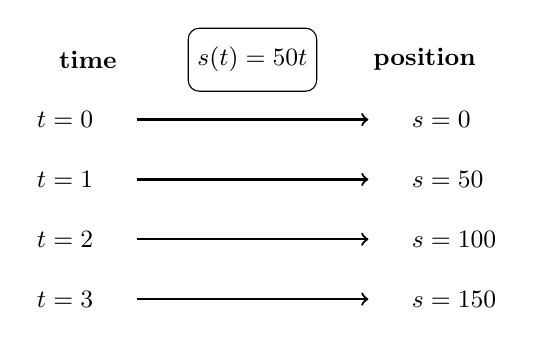
\begin{tikzpicture}[scale=0.95, every node/.style={font=\small}]
  \node at (-0.2,3.2) {\textbf{time}};
  \node at (4.3,3.2) {\textbf{position}};

  \foreach \y/\t/\s in {2.4/0/0,1.6/1/50,0.8/2/100,0/3/150} {
    \node[left] at (0,\y) {\(t=\t\)};
    \node[right] at (4,\y) {\(s=\s\)};
    \draw[->, thick] (0.45,\y) -- (3.55,\y);
  }

  \node[draw, rounded corners, align=center, minimum width=1.6cm, minimum height=0.8cm] at (2,3.2) {\(s(t)=50t\)};
\end{tikzpicture}
\caption{A function assigns an output to each input in its domain.}
\label{fig:function-assignment}
\end{figure}

The word ``assigns'' is important. A function is not merely a formula. It is a rule that gives exactly one output for each allowed input.

\begin{quote}
\textbf{Definition.}
A \emph{function} \(f\) from a set \(D\) to the real numbers is a rule that assigns to each input \(x\in D\) exactly one real number \(f(x)\).

The set \(D\) is called the \emph{domain} of \(f\).

The set of all outputs is called the \emph{range} of \(f\):

\[
\{f(x):x\in D\}.
\]
\end{quote}

We often write

\[
f:D\to \mathbb R.
\]

This means that the inputs come from \(D\), and the outputs are real numbers.

\paragraph{Example.}
Let

\[
f:\mathbb R\to \mathbb R,
\qquad
f(x)=x^2.
\]

The domain is all real numbers. The range is

\[
[0,\infty),
\]

because every square is nonnegative, and every nonnegative number is the square of some real number.

For instance, \(9\) is in the range because

\[
f(3)=9.
\]

But \(-4\) is not in the range because no real number has square \(-4\).

\paragraph{Same formula, different function.}
The formula alone does not always determine the function. Compare

\[
f:\mathbb R\to \mathbb R,
\qquad
f(x)=x^2,
\]

with

\[
g:[-1,1]\to \mathbb R,
\qquad
g(x)=x^2.
\]

The formulas are the same, but the domains are different. So the functions are different.

The range of \(f\) is

\[
[0,\infty),
\]

while the range of \(g\) is

\[
[0,1].
\]

A function is a rule together with its allowed inputs.

\subsection{Functions from formulas, graphs, tables, and words}
\label{subsec:functions-from-formulas-graphs-tables-words}

A formula is the most familiar way to describe a function, but it is not the only way.

\paragraph{A function from a formula.}
The area \(A\) of a circle depends on its radius \(r\):

\[
A(r)=\pi r^2.
\]

If the radius is measured in centimeters, then the area is measured in square centimeters. The natural domain is

\[
[0,\infty),
\]

because a radius cannot be negative.

\paragraph{A function from a table.}
A thermometer may record the temperature of a cup of tea every minute.

\[
\begin{array}{c|ccccc}
t\text{ (minutes)} & 0 & 1 & 2 & 3 & 4 \\ \hline
T(t)\text{ (degrees C)} & 90 & 82 & 75 & 69 & 64
\end{array}
\]

This table defines a function on the domain

\[
\{0,1,2,3,4\}.
\]

For example,

\[
T(2)=75.
\]

The table does not tell us the exact temperature at \(t=2.5\). It may suggest one, but it does not assign one unless we add more information.

This distinction will matter later. Data can suggest a model, but the model is a new function.

\paragraph{A function from a graph.}
A graph can also describe a function. The input \(x\) is read along the horizontal axis. The output \(f(x)\) is read along the vertical axis.

A graph represents a function only when each input gives exactly one output. This is the reason for the vertical line test: a vertical line corresponds to one input \(x\). If it hits a curve in two places, then that input has two possible outputs, so the curve is not the graph of a function of \(x\).

\begin{figure}[h]
\centering
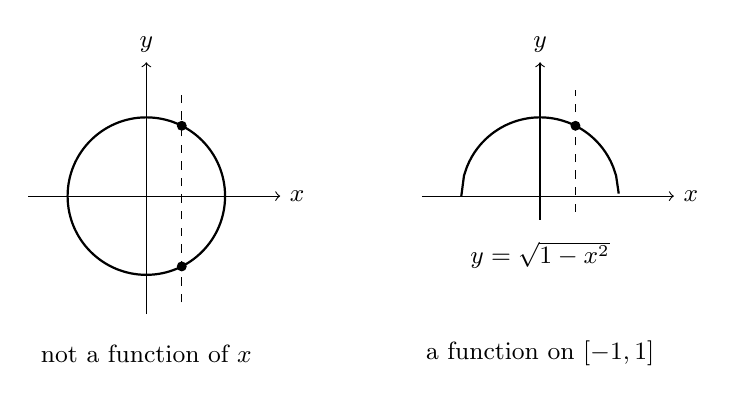
\begin{tikzpicture}[scale=1.0, every node/.style={font=\small}]
  % left: not a function
  \begin{scope}
    \draw[->] (-1.5,0) -- (1.7,0) node[right] {\(x\)};
    \draw[->] (0,-1.5) -- (0,1.7) node[above] {\(y\)};
    \draw[thick] (0,0) circle (1);
    \draw[dashed] (0.45,-1.35) -- (0.45,1.35);
    \fill (0.45,0.893) circle (1.8pt);
    \fill (0.45,-0.893) circle (1.8pt);
    \node at (0,-2.0) {not a function of \(x\)};
  \end{scope}

  % right: function
  \begin{scope}[xshift=5cm]
    \draw[->] (-1.5,0) -- (1.7,0) node[right] {\(x\)};
    \draw[->] (0,-0.3) -- (0,1.7) node[above] {\(y\)};
    \draw[thick, domain=-1:1, samples=60] plot (\x,{sqrt(1-\x*\x)});
    \draw[dashed] (0.45,-0.2) -- (0.45,1.35);
    \fill (0.45,0.893) circle (1.8pt);
    \node at (0,-0.75) {\(y=\sqrt{1-x^2}\)};
    \node at (0,-2.0) {a function on \([-1,1]\)};
  \end{scope}
\end{tikzpicture}
\caption{The full circle gives two \(y\)-values for many \(x\)-values. The upper semicircle gives exactly one.}
\label{fig:vertical-line-test}
\end{figure}

The circle

\[
x^2+y^2=1
\]

is not the graph of \(y\) as a function of \(x\), because most inputs \(x\) between \(-1\) and \(1\) give two outputs.

But the upper semicircle

\[
y=\sqrt{1-x^2}
\]

is a function on the domain \([-1,1]\).

\paragraph{A function from words.}
Sometimes the rule is best described in words.

For example:

\[
C(m)=\text{the cost, in dollars, of a taxi ride of }m\text{ miles}.
\]

A simple model might be

\[
C(m)=4+2.50m.
\]

Here \(4\) is the starting charge, and \(2.50\) is the cost per mile. The units help us read the formula:

\[
2.50\frac{\text{dollars}}{\text{mile}}\cdot m\text{ miles}
=
2.50m\text{ dollars}.
\]

The natural domain is

\[
[0,\infty),
\]

or perhaps a smaller interval if the taxi company serves only local trips.

\begin{quote}
\textbf{A useful habit.}
When you meet a function, ask four questions:

\[
\text{What are the inputs?}
\]

\[
\text{What are the outputs?}
\]

\[
\text{What units do they have?}
\]

\[
\text{What inputs are allowed?}
\]
\end{quote}

\subsection{The natural domain of a formula}
\label{subsec:natural-domain-formula}

When a formula is given without an explicit domain, we usually take the domain to be all real numbers for which the formula makes sense. This is called the \emph{natural domain}.

\paragraph{Example.}
For

\[
f(x)=\frac{1}{x-2},
\]

the denominator cannot be \(0\). Therefore

\[
x\neq 2.
\]

The natural domain is

\[
(-\infty,2)\cup(2,\infty).
\]

\paragraph{Example.}
For

\[
g(x)=\sqrt{x-1},
\]

the quantity under the square root must be nonnegative:

\[
x-1\ge 0.
\]

So

\[
x\ge 1,
\]

and the natural domain is

\[
[1,\infty).
\]

\paragraph{Example.}
For

\[
h(x)=\sqrt{4-x^2},
\]

we need

\[
4-x^2\ge 0.
\]

This means

\[
x^2\le 4,
\]

so

\[
-2\le x\le 2.
\]

The natural domain is

\[
[-2,2].
\]

In fact, the graph of

\[
y=\sqrt{4-x^2}
\]

is the upper half of the circle

\[
x^2+y^2=4.
\]

The domain is the horizontal interval covered by the semicircle. The range is

\[
[0,2].
\]

\subsection{Piecewise-defined functions}
\label{subsec:piecewise-functions}

Many real processes follow one rule for a while and then another rule later.

A car may move forward, stop at a light, then reverse into a parking space. A tax bill may use one rate for the first part of income and another rate for the next part. A postage cost may stay constant over a range of weights, then jump.

These functions are often described piece by piece.

\paragraph{Example: forward, then backward.}
A car starts at position \(0\), moves forward at \(40\) miles/hour for \(2\) hours, and then moves backward at \(30\) miles/hour for \(1\) hour.

For \(0\le t\le 2\), the position is

\[
s(t)=40t.
\]

At \(t=2\), the car has reached

\[
s(2)=80.
\]

After that, the car moves backward at \(30\) miles/hour. For \(2<t\le 3\), its position is

\[
s(t)=80-30(t-2).
\]

Thus

\[
s(t)=
\begin{cases}
40t, & 0\le t\le 2,\\
80-30(t-2), & 2<t\le 3.
\end{cases}
\]

The domain is

\[
[0,3].
\]

The range is

\[
[0,80],
\]

because the car starts at \(0\), reaches \(80\), and then returns to \(50\).

\begin{figure}[h]
\centering
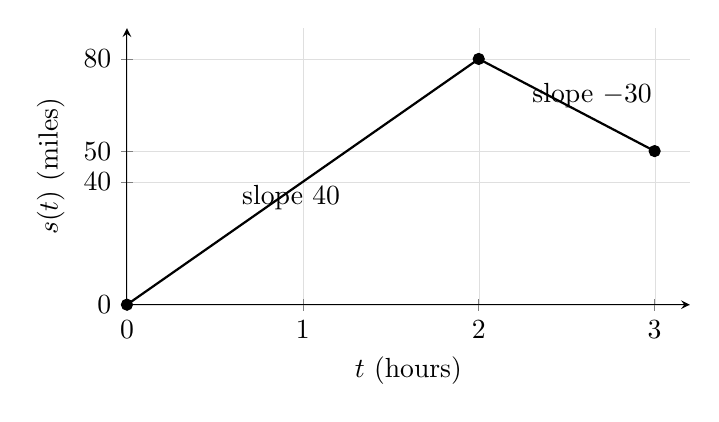
\begin{tikzpicture}
\begin{axis}[
    width=0.72\textwidth,
    height=0.42\textwidth,
    xmin=0, xmax=3.2,
    ymin=0, ymax=90,
    axis lines=left,
    xlabel={\(t\) (hours)},
    ylabel={\(s(t)\) (miles)},
    xtick={0,1,2,3},
    ytick={0,40,50,80},
    grid=both,
    grid style={line width=.1pt, draw=gray!25},
]
\addplot[thick, domain=0:2, samples=2] {40*x};
\addplot[thick, domain=2:3, samples=2] {80-30*(x-2)};
\addplot[only marks,mark=*] coordinates {(0,0) (2,80) (3,50)};
\node[anchor=west] at (axis cs:0.6,35) {slope \(40\)};
\node[anchor=west] at (axis cs:2.25,68) {slope \(-30\)};
\end{axis}
\end{tikzpicture}
\caption{A piecewise function can describe motion whose rule changes.}
\label{fig:piecewise-position-function}
\end{figure}

At \(t=2\), the definition uses only the first formula. That is enough. A function must give one output for each input, not two.

Here the second formula would also give

\[
80-30(2-2)=80,
\]

so there would be no conflict if we included \(t=2\) in both pieces. But it is cleaner to assign the boundary point once.

\paragraph{A warning.}
The expression

\[
F(x)=
\begin{cases}
1, & x\le 0,\\
2, & x\ge 0
\end{cases}
\]

does not define a function, because at \(x=0\) it assigns two outputs:

\[
F(0)=1
\quad\text{and}\quad
F(0)=2.
\]

To make it a function, one of the pieces must give up the endpoint. For example,

\[
F(x)=
\begin{cases}
1, & x<0,\\
2, & x\ge 0
\end{cases}
\]

is a function.

This small detail matters. Calculus often studies what happens near a boundary point, so we must know exactly what value the function has there.

\subsection{The difference quotient as a function of two inputs}
\label{subsec:difference-quotient-function}

Chapter 1 already used expressions such as

\[
\frac{s(2+h)-s(2)}{h}.
\]

This is an average velocity over a short interval. It is also a new function built from the old function \(s\).

For a general function \(f\), a base input \(a\), and a nonzero step \(h\), define

\[
Q_f(a,h)=\frac{f(a+h)-f(a)}{h}.
\]

This is called a \emph{difference quotient}.

The input \(a\) tells us where we start. The input \(h\) tells us how far we step. The output is the average rate of change from \(a\) to \(a+h\).

\[
Q_f(a,h)
=
\frac{\text{change in output}}{\text{change in input}}.
\]

The condition

\[
h\neq 0
\]

is necessary because division by \(0\) is not allowed.

There is another domain condition too: both \(a\) and \(a+h\) must be in the domain of \(f\).

\paragraph{Example.}
Let

\[
f(x)=x^2.
\]

Then

\[
Q_f(a,h)
=
\frac{(a+h)^2-a^2}{h}.
\]

For \(h\neq 0\),

\[
Q_f(a,h)
=
\frac{a^2+2ah+h^2-a^2}{h}
=
\frac{2ah+h^2}{h}
=
2a+h.
\]

So for the square function,

\[
\boxed{Q_f(a,h)=2a+h,\qquad h\neq 0.}
\]

If \(a=2\), then

\[
Q_f(2,h)=4+h.
\]

This is exactly the expression from Chapter 1. As \(h\) becomes small, the average rate \(4+h\) gets close to \(4\).

\begin{figure}[h]
\centering
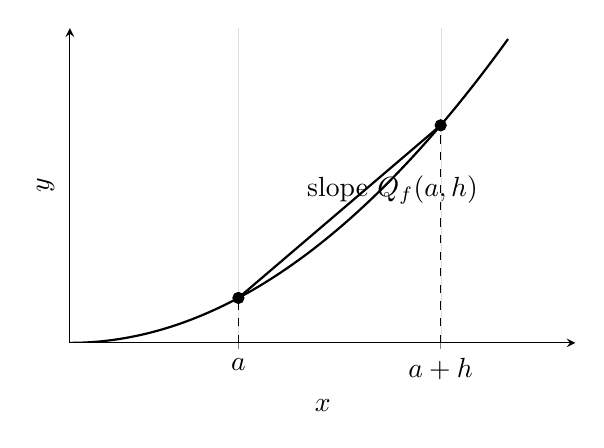
\begin{tikzpicture}
\begin{axis}[
    width=0.66\textwidth,
    height=0.46\textwidth,
    xmin=0, xmax=3,
    ymin=0, ymax=7,
    axis lines=left,
    xlabel={\(x\)},
    ylabel={\(y\)},
    xtick={1,2.2},
    xticklabels={\(a\),\(a+h\)},
    ytick=\empty,
    grid=both,
    grid style={line width=.1pt, draw=gray!25},
]
\addplot[thick, domain=0:2.6, samples=80] {x^2};
\addplot[thick] coordinates {(1,1) (2.2,4.84)};
\addplot[only marks,mark=*] coordinates {(1,1) (2.2,4.84)};
\draw[dashed] (axis cs:1,0) -- (axis cs:1,1);
\draw[dashed] (axis cs:2.2,0) -- (axis cs:2.2,4.84);
\node[anchor=west] at (axis cs:1.35,3.4) {slope \(Q_f(a,h)\)};
\end{axis}
\end{tikzpicture}
\caption{The difference quotient is the slope of the secant line through the points with inputs \(a\) and \(a+h\).}
\label{fig:difference-quotient-secant}
\end{figure}

\paragraph{Example: domain restrictions in the difference quotient.}
Let

\[
f(x)=\sqrt{x}.
\]

The domain of \(f\) is

\[
[0,\infty).
\]

For

\[
Q_f(a,h)=\frac{\sqrt{a+h}-\sqrt a}{h},
\]

we need

\[
a\ge 0,\qquad a+h\ge 0,\qquad h\neq 0.
\]

So the difference quotient has a domain of its own. It is not enough to say ``\(h\neq 0\).'' We must also keep both inputs of \(f\) legal.

\begin{quote}
\textbf{Why this matters.}
The derivative will come from the difference quotient by letting \(h\) move toward \(0\). Before taking that limit, we need to know where the quotient is defined.
\end{quote}

Functions let one quantity depend on another. Graphs let us see that dependence all at once. Before we can study limits on graphs, we need to learn how graphs move, stretch, reflect, and reveal information.

\section{Graphs and transformations}
\label{sec:graphs-transformations}

A function is an assignment. A graph is a picture of all those assignments at once.

Each point on the graph of \(y=f(x)\) has the form

\[
(x,f(x)).
\]

The horizontal coordinate is the input. The vertical coordinate is the output.

A graph can show things a formula hides: where a function is positive, where it is zero, where it grows large, and where it has symmetry. It also helps us build new functions from old ones.

\subsection{Shifts and scalings}
\label{subsec:shifts-and-scalings}

Start with the simplest curved graph:

\[
f(x)=x^2.
\]

Its graph is a parabola. Now compare it with

\[
g(x)=f(x)+3=x^2+3.
\]

For every input \(x\), the output of \(g\) is \(3\) more than the output of \(f\). So every point of the graph moves up \(3\) units.

\[
(x,f(x))
\quad\longmapsto\quad
(x,f(x)+3).
\]

Thus \(y=x^2+3\) is the graph of \(y=x^2\) shifted upward by \(3\).

Now compare \(f(x)=x^2\) with

\[
h(x)=f(x-2)=(x-2)^2.
\]

This one is more subtle. The graph shifts to the right, not to the left.

Why? The old function \(f\) has its lowest point at input \(0\), because

\[
f(0)=0.
\]

The new function \(h\) has its lowest point when the inside input is \(0\):

\[
x-2=0.
\]

So

\[
x=2.
\]

The point \((0,0)\) on the old graph becomes \((2,0)\) on the new graph.

\begin{figure}[h]
\centering
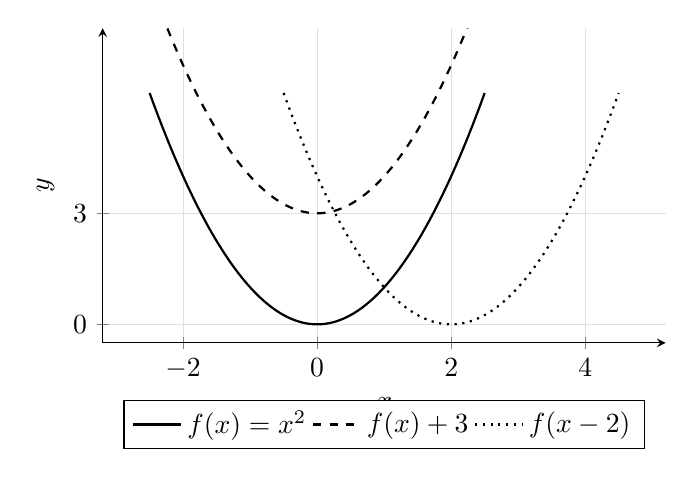
\begin{tikzpicture}
\begin{axis}[
    width=0.72\textwidth,
    height=0.46\textwidth,
    xmin=-3.2, xmax=5.2,
    ymin=-0.5, ymax=8,
    axis lines=left,
    xlabel={\(x\)},
    ylabel={\(y\)},
    xtick={-2,0,2,4},
    ytick={0,3},
    grid=both,
    grid style={line width=.1pt, draw=gray!25},
    legend style={at={(0.5,-0.18)},anchor=north,legend columns=3}
]
\addplot[thick, domain=-2.5:2.5, samples=80] {x^2};
\addlegendentry{\(f(x)=x^2\)}
\addplot[thick, dashed, domain=-2.5:2.5, samples=80] {x^2+3};
\addlegendentry{\(f(x)+3\)}
\addplot[thick, dotted, domain=-0.5:4.5, samples=80] {(x-2)^2};
\addlegendentry{\(f(x-2)\)}
\end{axis}
\end{tikzpicture}
\caption{Adding outside the function shifts vertically. Changing the input inside the function shifts horizontally.}
\label{fig:vertical-horizontal-shifts}
\end{figure}

\begin{quote}
\textbf{Shifts.}
For \(c>0\):

\[
y=f(x)+c
\]

shifts the graph of \(y=f(x)\) upward by \(c\).

\[
y=f(x)-c
\]

shifts it downward by \(c\).

\[
y=f(x-c)
\]

shifts it right by \(c\).

\[
y=f(x+c)
\]

shifts it left by \(c\).
\end{quote}

Horizontal shifts often feel backward at first. The reason is that the expression inside the function asks:

\[
\text{What input should the old function receive?}
\]

If the new input must satisfy \(x-c=a\), then \(x=a+c\). So old input \(a\) appears \(c\) units to the right.

\paragraph{Example.}
Let

\[
f(x)=\sqrt{x}.
\]

Then

\[
g(x)=\sqrt{x-4}
\]

is the graph of \(f\) shifted right by \(4\).

The domain also shifts. The old domain is

\[
[0,\infty).
\]

The new function requires

\[
x-4\ge 0,
\]

so

\[
x\ge 4.
\]

Thus the domain of \(g\) is

\[
[4,\infty).
\]

\subsection{Reflections and stretching}
\label{subsec:reflections-and-stretching}

A vertical scaling changes the outputs.

For example, if

\[
f(x)=x^2,
\]

then

\[
g(x)=2f(x)=2x^2.
\]

Every output doubles. A point

\[
(a,f(a))
\]

moves to

\[
(a,2f(a)).
\]

The graph is stretched vertically by a factor of \(2\).

If

\[
g(x)=\frac12 f(x),
\]

then every output is cut in half. The graph is compressed vertically by a factor of \(2\).

Horizontal scaling changes the inputs. For example,

\[
h(x)=f(2x).
\]

The output that used to occur at input \(a\) now occurs when

\[
2x=a,
\]

so

\[
x=\frac a2.
\]

The graph is compressed horizontally by a factor of \(2\).

\begin{quote}
\textbf{Scaling rules.}
For \(A>0\), the graph of

\[
y=Af(x)
\]

is a vertical scaling of the graph of \(y=f(x)\) by factor \(A\).

For \(B>0\), the graph of

\[
y=f(Bx)
\]

is a horizontal scaling by factor \(\frac1B\).
\end{quote}

Again, changes inside the function work in the opposite direction from what the eye may expect. The input \(Bx\) reaches old values \(B\) times as fast, so the graph is squeezed horizontally when \(B>1\).

\paragraph{Example.}
Let

\[
f(x)=\sin x.
\]

Then

\[
g(x)=\sin(2x)
\]

runs through one full sine wave twice as fast as \(\sin x\). Its period is

\[
\pi
\]

instead of

\[
2\pi.
\]

The graph is compressed horizontally by a factor of \(2\).

Reflections are special scalings by \(-1\).

The graph of

\[
y=-f(x)
\]

is the reflection of \(y=f(x)\) across the \(x\)-axis. Every output changes sign:

\[
(a,f(a))
\quad\longmapsto\quad
(a,-f(a)).
\]

The graph of

\[
y=f(-x)
\]

is the reflection of \(y=f(x)\) across the \(y\)-axis. Every input changes sign:

\[
(a,f(a))
\quad\longmapsto\quad
(-a,f(a)).
\]

\begin{center}
\[
\begin{array}{c|c|c}
\textbf{new function} & \textbf{point movement} & \textbf{graph effect} \\ \hline
f(x)+k & (a,f(a))\mapsto(a,f(a)+k) & \text{vertical shift} \\
f(x-c) & (a,f(a))\mapsto(a+c,f(a)) & \text{horizontal shift} \\
Af(x) & (a,f(a))\mapsto(a,Af(a)) & \text{vertical scaling} \\
f(Bx),\ B>0 & (a,f(a))\mapsto(a/B,f(a)) & \text{horizontal scaling} \\
-f(x) & (a,f(a))\mapsto(a,-f(a)) & \text{reflection across \(x\)-axis} \\
f(-x) & (a,f(a))\mapsto(-a,f(a)) & \text{reflection across \(y\)-axis}
\end{array}
\]
\end{center}

\paragraph{Example: the order matters.}
Let

\[
f(x)=x^2.
\]

Compare

\[
g(x)=2f(x-3)
\]

with

\[
r(x)=2f(x)-3.
\]

The first function is

\[
g(x)=2(x-3)^2.
\]

It shifts the parabola right by \(3\), then stretches vertically by \(2\).

The second function is

\[
r(x)=2x^2-3.
\]

It stretches vertically by \(2\), then shifts downward by \(3\).

These are not the same function. For example,

\[
g(0)=2(0-3)^2=18,
\]

but

\[
r(0)=2\cdot 0^2-3=-3.
\]

Small changes in the formula can mean different geometric changes.

\subsection{Even and odd symmetry}
\label{subsec:even-odd-symmetry}

Some graphs have symmetry around the vertical axis. Others have symmetry around the origin.

The function

\[
f(x)=x^2
\]

satisfies

\[
f(-x)=(-x)^2=x^2=f(x).
\]

So the outputs at \(x\) and \(-x\) are the same. The graph is symmetric across the \(y\)-axis.

The function

\[
g(x)=x^3
\]

satisfies

\[
g(-x)=(-x)^3=-x^3=-g(x).
\]

So the output at \(-x\) is the negative of the output at \(x\). The graph has origin symmetry: rotating it \(180^\circ\) around the origin gives the same graph.

\begin{figure}[h]
\centering
\begin{minipage}{0.47\textwidth}
\centering
\begin{tikzpicture}
\begin{axis}[
    width=\textwidth,
    height=0.72\textwidth,
    xmin=-2.2, xmax=2.2,
    ymin=-0.5, ymax=4.5,
    axis lines=middle,
    xlabel={\(x\)},
    ylabel={\(y\)},
    xtick={-2,-1,0,1,2},
    ytick={0,1,4},
    grid=both,
    grid style={line width=.1pt, draw=gray!25},
]
\addplot[thick, domain=-2:2, samples=80] {x^2};
\node[anchor=west] at (axis cs:0.4,3.5) {\(y=x^2\)};
\end{axis}
\end{tikzpicture}
\end{minipage}
\hfill
\begin{minipage}{0.47\textwidth}
\centering
\begin{tikzpicture}
\begin{axis}[
    width=\textwidth,
    height=0.72\textwidth,
    xmin=-2.2, xmax=2.2,
    ymin=-5, ymax=5,
    axis lines=middle,
    xlabel={\(x\)},
    ylabel={\(y\)},
    xtick={-2,-1,0,1,2},
    ytick={-4,0,4},
    grid=both,
    grid style={line width=.1pt, draw=gray!25},
]
\addplot[thick, domain=-1.65:1.65, samples=80] {x^3};
\node[anchor=west] at (axis cs:0.45,3.6) {\(y=x^3\)};
\end{axis}
\end{tikzpicture}
\end{minipage}
\caption{The square function is even. The cube function is odd.}
\label{fig:even-odd-basic}
\end{figure}

\begin{quote}
\textbf{Definition.}
Suppose the domain of \(f\) is symmetric about \(0\): whenever \(x\) is in the domain, so is \(-x\).

The function \(f\) is \emph{even} if

\[
f(-x)=f(x)
\]

for every \(x\) in the domain.

The function \(f\) is \emph{odd} if

\[
f(-x)=-f(x)
\]

for every \(x\) in the domain.
\end{quote}

\paragraph{Examples.}
The functions

\[
x^2,\qquad x^4,\qquad \cos x
\]

are even.

The functions

\[
x,\qquad x^3,\qquad \sin x
\]

are odd.

The function

\[
f(x)=x^2+x
\]

is neither even nor odd, because

\[
f(-x)=x^2-x,
\]

which is not equal to \(f(x)=x^2+x\), and is not equal to \(-f(x)=-x^2-x\).

\paragraph{A small consequence.}
If \(f\) is odd and \(0\) is in its domain, then

\[
f(0)=0.
\]

Indeed,

\[
f(-0)=-f(0).
\]

But \(-0=0\), so

\[
f(0)=-f(0).
\]

Thus

\[
2f(0)=0,
\]

and therefore

\[
f(0)=0.
\]

So an odd function whose graph includes \(x=0\) must pass through the origin.

Symmetry is not only pretty. It saves work. If an even function is known for \(x\ge 0\), then it is known for \(x\le 0\). If an odd function is known for \(x\ge 0\), then the other half is determined by sign change.

\subsection{Reading intercepts, sign, and intervals from a graph}
\label{subsec:reading-intercepts-sign-intervals}

A graph is a picture of outputs. But many questions about a function are really questions about intervals of inputs.

\[
\text{Where is }f(x)=0?
\]

\[
\text{Where is }f(x)>0?
\]

\[
\text{Where is }f(x)<0?
\]

\[
\text{Which inputs are allowed?}
\]

\[
\text{Which outputs occur?}
\]

The graph answers these questions visually.

\begin{quote}
\textbf{Reading a graph.}

The \emph{domain} is the set of \(x\)-values covered by the graph.

The \emph{range} is the set of \(y\)-values reached by the graph.

The \emph{\(x\)-intercepts} are the points where the graph crosses or touches the \(x\)-axis. They occur when

\[
f(x)=0.
\]

The \emph{\(y\)-intercept} occurs at

\[
x=0,
\]

if \(0\) is in the domain.

The function is positive where the graph lies above the \(x\)-axis, and negative where it lies below the \(x\)-axis.
\end{quote}

\paragraph{Example.}
Consider

\[
p(x)=\frac15(x+2)(x-1)(x-3).
\]

The zeros are visible from the factored form:

\[
x=-2,\qquad x=1,\qquad x=3.
\]

These are the \(x\)-intercepts.

The \(y\)-intercept is

\[
p(0)=\frac15(2)(-1)(-3)=\frac65.
\]

So the graph crosses the \(y\)-axis at

\[
\left(0,\frac65\right).
\]

\begin{figure}[h]
\centering
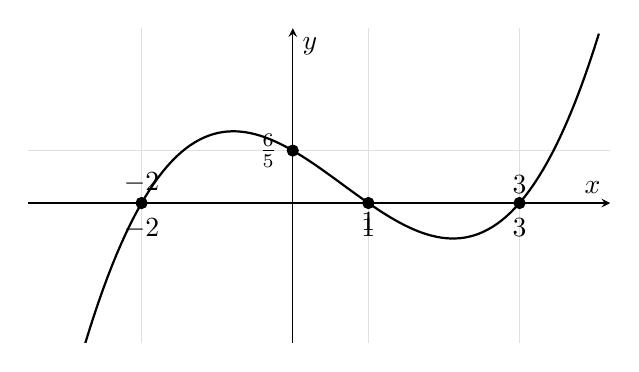
\begin{tikzpicture}
\begin{axis}[
    width=0.74\textwidth,
    height=0.46\textwidth,
    xmin=-3.5, xmax=4.2,
    ymin=-3.2, ymax=4,
    axis lines=middle,
    xlabel={\(x\)},
    ylabel={\(y\)},
    xtick={-2,0,1,3},
    ytick={0,1.2},
    yticklabels={\(0\),\(\frac65\)},
    grid=both,
    grid style={line width=.1pt, draw=gray!25},
]
\addplot[thick, domain=-3.25:4.05, samples=120] {0.2*(x+2)*(x-1)*(x-3)};
\addplot[only marks,mark=*] coordinates {(-2,0) (1,0) (3,0) (0,1.2)};
\node[anchor=south] at (axis cs:-2,0) {\(-2\)};
\node[anchor=north] at (axis cs:1,0) {\(1\)};
\node[anchor=south] at (axis cs:3,0) {\(3\)};
\end{axis}
\end{tikzpicture}
\caption{Zeros divide the \(x\)-axis into intervals. On each interval, the graph is either above or below the axis until it crosses again.}
\label{fig:cubic-sign-intervals}
\end{figure}

The zeros divide the real line into four intervals:

\[
(-\infty,-2),\qquad (-2,1),\qquad (1,3),\qquad (3,\infty).
\]

From the graph, or from the signs of the factors, we find:

\[
\begin{array}{c|c}
\textbf{interval} & \textbf{sign of }p(x) \\ \hline
(-\infty,-2) & p(x)<0 \\
(-2,1) & p(x)>0 \\
(1,3) & p(x)<0 \\
(3,\infty) & p(x)>0
\end{array}
\]

Notice the difference between a point and an interval:

\[
p(-2)=0
\]

is a statement about one input.

\[
p(x)>0 \text{ on }(-2,1)
\]

is a statement about infinitely many inputs.

Calculus will often turn a question about a whole graph into questions about intervals. Where is the function increasing? Where is it decreasing? Where is it concave up? Where does it have a largest value?

For now, we only need the first graph-reading skills: intercepts, sign, domain, range, and transformations.

\subsection{A graph can suggest, but not prove}
\label{subsec:graph-suggest-not-prove}

Graphs are honest when drawn carefully, but they are not proofs by themselves.

A graphing window can hide behavior. A curve may cross the axis just outside the window. A tiny wiggle may disappear if the scale is too large. A vertical asymptote may look like a steep line.

For example, the functions

\[
f(x)=x^2
\]

and

\[
g(x)=x^2+0.001\sin(1000x)
\]

can look almost identical in a wide viewing window. But the second function has many small oscillations.

The lesson is not to distrust graphs. The lesson is to use them correctly.

\begin{quote}
\textbf{Graphs guide the eye. Algebra and definitions check the claim.}
\end{quote}

Transformations let us build many new functions from one familiar function. Next we will build functions in a more algebraic way: by adding, multiplying, dividing, and composing them. Composition is the most hidden of these operations, and later it will force one of the most important derivative rules in calculus.
\section{Combining functions}
\label{sec:combining-functions}

Transformations moved a graph without changing its basic identity. A parabola could shift, stretch, or reflect and still be built from the same old rule.

There is another way to make new functions. We can combine outputs. We can multiply two changing quantities. We can divide one quantity by another. Most importantly, we can feed the output of one function into the input of another.

These operations are not bookkeeping. Later, each one will force a derivative rule.

\subsection{Sums, products, and quotients}
\label{subsec:sums-products-quotients}

Suppose a small delivery company charges for a trip in two parts. The driver cost is

\[
D(m)=25+0.40m,
\]

where \(m\) is the number of miles. The fuel cost is

\[
F(m)=0.18m.
\]

Both functions have the same input: miles. The total cost is therefore

\[
C(m)=D(m)+F(m).
\]

So

\[
C(m)=25+0.40m+0.18m=25+0.58m.
\]

This is a new function made from two old ones.

The same idea works in general.

\begin{quote}
\textbf{Arithmetic of functions.}
If \(f\) and \(g\) are functions, then we define

\[
(f+g)(x)=f(x)+g(x),
\]

\[
(f-g)(x)=f(x)-g(x),
\]

\[
(fg)(x)=f(x)g(x),
\]

and, when \(g(x)\neq 0\),

\[
\left(\frac{f}{g}\right)(x)=\frac{f(x)}{g(x)}.
\]
\end{quote}

The input \(x\) must be allowed for both functions. For the quotient, we also need the denominator not to be zero.

\paragraph{Example: a domain is part of the answer.}
Let

\[
f(x)=\sqrt{x}
\]

and

\[
g(x)=\frac{1}{x-2}.
\]

The domain of \(f\) is

\[
[0,\infty),
\]

and the domain of \(g\) is

\[
(-\infty,2)\cup(2,\infty).
\]

Therefore the domain of \(f+g\) is the overlap:

\[
[0,\infty)\cap\left((-\infty,2)\cup(2,\infty)\right).
\]

So

\[
\operatorname{domain}(f+g)=[0,2)\cup(2,\infty).
\]

On that domain,

\[
(f+g)(x)=\sqrt{x}+\frac{1}{x-2}.
\]

The same domain is used for the product

\[
(fg)(x)=\frac{\sqrt{x}}{x-2}.
\]

A formula may look harmless, but the old restrictions remain.

\paragraph{Example: multiplying two changing quantities.}
A rectangle has length

\[
\ell(t)=3+t
\]

and width

\[
w(t)=5-2t,
\]

where \(t\) is time in seconds. Its area is

\[
A(t)=\ell(t)w(t).
\]

Thus

\[
A(t)=(3+t)(5-2t).
\]

Expanding,

\[
A(t)=15-t-2t^2.
\]

But the physical domain is not all real numbers. Length and width should be nonnegative:

\[
3+t\ge 0
\]

and

\[
5-2t\ge 0.
\]

So

\[
t\ge -3
\qquad\text{and}\qquad
t\le \frac52.
\]

The physical domain is

\[
\left[-3,\frac52\right].
\]

Algebra alone produced the formula. The meaning of the variables produced the domain.

\paragraph{A warning about cancellation.}
Consider

\[
h(x)=\frac{x^2-1}{x-1}.
\]

Because

\[
x^2-1=(x-1)(x+1),
\]

we can simplify:

\[
h(x)=x+1,
\qquad x\neq 1.
\]

The condition \(x\neq 1\) cannot be erased. The original formula was not defined at \(x=1\). So \(h\) is not the same function as

\[
p(x)=x+1
\]

with domain all real numbers.

They have the same values for every \(x\neq 1\), but they do not have the same domain.

\begin{quote}
\textbf{Moral.}
Simplifying a formula can hide a missing input. A function is not only a formula; it is a formula together with its allowed inputs.
\end{quote}

This small warning will return when we study limits. Sometimes a function has a hole at one point, but its nearby values still point clearly toward a missing height.

\subsection{Composition}
\label{subsec:composition}

Addition, multiplication, and division combine outputs that come from the same input. Composition is different. In composition, the output of one function becomes the input of another.

Imagine a hiker walking along a straight trail. At time \(t\), her position is

\[
s(t)=3t
\]

miles from the trailhead. The temperature at position \(x\) miles from the trailhead is

\[
T(x)=70-2x
\]

degrees Fahrenheit.

What is the temperature around the hiker at time \(t\)?

First time gives position:

\[
t\mapsto s(t)=3t.
\]

Then position gives temperature:

\[
x\mapsto T(x)=70-2x.
\]

So time gives temperature by two steps:

\[
T(s(t))=T(3t)=70-2(3t)=70-6t.
\]

This is a composition.

\begin{figure}[h]
\centering
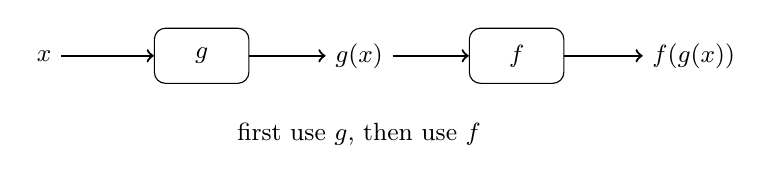
\begin{tikzpicture}[every node/.style={font=\small}]
  \node (x) at (0,0) {\(x\)};
  \node[draw, rounded corners, minimum width=1.2cm, minimum height=0.7cm] (g) at (2,0) {\(g\)};
  \node (gx) at (4,0) {\(g(x)\)};
  \node[draw, rounded corners, minimum width=1.2cm, minimum height=0.7cm] (f) at (6,0) {\(f\)};
  \node (fgx) at (8.25,0) {\(f(g(x))\)};

  \draw[->, thick] (x) -- (g);
  \draw[->, thick] (g) -- (gx);
  \draw[->, thick] (gx) -- (f);
  \draw[->, thick] (f) -- (fgx);

  \node at (4,-1.0) {first use \(g\), then use \(f\)};
\end{tikzpicture}
\caption{In \(f(g(x))\), the function \(g\) acts first. Its output becomes the input of \(f\).}
\label{fig:composition-machine}
\end{figure}

\begin{quote}
\textbf{Definition.}
The \emph{composition} of \(f\) with \(g\) is the function

\[
(f\circ g)(x)=f(g(x)).
\]

The function \(g\) is applied first. The function \(f\) is applied second.
\end{quote}

The symbol \(f\circ g\) is read ``\(f\) composed with \(g\).''

The order matters. Usually,

\[
f\circ g \neq g\circ f.
\]

\paragraph{Example: order matters.}
Let

\[
f(u)=\sqrt{u}
\]

and

\[
g(x)=4-x^2.
\]

Then

\[
(f\circ g)(x)=f(g(x))=\sqrt{4-x^2}.
\]

For this to make sense, we need

\[
4-x^2\ge 0.
\]

So

\[
-2\le x\le 2.
\]

Thus

\[
\operatorname{domain}(f\circ g)=[-2,2].
\]

Now reverse the order:

\[
(g\circ f)(x)=g(f(x))=4-(\sqrt{x})^2.
\]

This simplifies to

\[
4-x,
\]

but only for inputs where \(\sqrt{x}\) is defined. Therefore

\[
\operatorname{domain}(g\circ f)=[0,\infty).
\]

So

\[
f\circ g
\]

and

\[
g\circ f
\]

are different functions.

\begin{quote}
\textbf{Domain of a composition.}
For \(f(g(x))\) to be defined, two things must happen:

\[
x \text{ must be allowed as an input of } g,
\]

and

\[
g(x) \text{ must be allowed as an input of } f.
\]

In symbols,

\[
\operatorname{domain}(f\circ g)
=
\{x\in \operatorname{domain}(g): g(x)\in \operatorname{domain}(f)\}.
\]
\end{quote}

\paragraph{Example: composition inside a transformation.}
The function

\[
h(x)=(x-2)^2
\]

can be read as a composition.

Let

\[
g(x)=x-2
\]

and

\[
f(u)=u^2.
\]

Then

\[
h(x)=f(g(x)).
\]

First subtract \(2\). Then square.

This is why horizontal shifts can feel backward. The inside function changes the input before the outer function sees it.

\subsection{Inverse functions}
\label{subsec:inverse-functions}

Some functions can be undone.

Temperature conversion gives a simple example. If \(C\) is temperature in degrees Celsius, then the corresponding Fahrenheit temperature is

\[
F(C)=\frac95 C+32.
\]

For example,

\[
F(20)=\frac95(20)+32=68.
\]

If we know the Fahrenheit temperature and want Celsius, we solve

\[
F=\frac95 C+32.
\]

Subtract \(32\):

\[
F-32=\frac95 C.
\]

Multiply by \(\frac59\):

\[
C=\frac59(F-32).
\]

So the function that undoes \(F(C)\) is

\[
C(F)=\frac59(F-32).
\]

Check:

\[
C(F(20))
=
\frac59(68-32)
=
20.
\]

The two conversions undo each other.

\begin{quote}
\textbf{Definition.}
Suppose \(f\) is a function with domain \(D\) and range \(R_f\). An \emph{inverse function} for \(f\) is a function

\[
f^{-1}:R_f\to D
\]

such that

\[
f^{-1}(f(x))=x
\]

for every \(x\in D\), and

\[
f(f^{-1}(y))=y
\]

for every \(y\in R_f\).
\end{quote}

The notation \(f^{-1}\) is read ``\(f\) inverse.''

It does not mean reciprocal. In general,

\[
f^{-1}(x)\neq \frac{1}{f(x)}.
\]

For example, if

\[
f(x)=x+3,
\]

then

\[
f^{-1}(x)=x-3,
\]

not

\[
\frac{1}{x+3}.
\]

\paragraph{Example.}
Let

\[
f(x)=2x-7.
\]

To find the inverse, write

\[
y=2x-7
\]

and solve for \(x\):

\[
y+7=2x,
\]

so

\[
x=\frac{y+7}{2}.
\]

Therefore

\[
f^{-1}(y)=\frac{y+7}{2}.
\]

Using \(x\) as the input variable for the inverse, we write

\[
f^{-1}(x)=\frac{x+7}{2}.
\]

Check both directions:

\[
f^{-1}(f(x))
=
\frac{(2x-7)+7}{2}
=
x,
\]

and

\[
f(f^{-1}(x))
=
2\left(\frac{x+7}{2}\right)-7
=
x.
\]

\subsection{When an inverse exists}
\label{subsec:when-inverse-exists}

Not every function can be undone.

The problem is duplication. If two different inputs give the same output, then the output does not remember which input produced it.

The square function on all real numbers is the first example:

\[
f(x)=x^2.
\]

It sends both \(2\) and \(-2\) to \(4\):

\[
f(2)=4,
\qquad
f(-2)=4.
\]

An inverse would have to answer the question:

\[
f^{-1}(4)=?
\]

Should the answer be \(2\) or \(-2\)? A function is allowed only one output for each input, so there is no inverse function for \(x^2\) on all of \(\mathbb R\).

\begin{quote}
\textbf{Definition.}
A function \(f\) is \emph{one-to-one} if different inputs always give different outputs.

Equivalently,

\[
f(x_1)=f(x_2)
\quad\Longrightarrow\quad
x_1=x_2.
\]
\end{quote}

\begin{quote}
\textbf{Inverse criterion.}
A function has an inverse function exactly when it is one-to-one.
\end{quote}

\paragraph{Why this is true.}
If \(f\) has an inverse, then one output cannot come from two different inputs. For if

\[
f(x_1)=f(x_2),
\]

then applying \(f^{-1}\) to both sides gives

\[
f^{-1}(f(x_1))=f^{-1}(f(x_2)).
\]

Therefore

\[
x_1=x_2.
\]

So \(f\) is one-to-one.

Conversely, if \(f\) is one-to-one, then every output in the range came from exactly one input. We can define \(f^{-1}(y)\) to be that unique input. That gives an inverse function.

\paragraph{The horizontal line test.}
A graph represents a one-to-one function exactly when every horizontal line crosses the graph at most once.

A horizontal line represents one output value. If it hits the graph twice, then two different inputs produced the same output. That prevents an inverse.

\begin{figure}[h]
\centering
\begin{minipage}{0.47\textwidth}
\centering
\begin{tikzpicture}
\begin{axis}[
    width=\textwidth,
    height=0.78\textwidth,
    xmin=-2.6, xmax=2.6,
    ymin=-0.5, ymax=6,
    axis lines=middle,
    xlabel={\(x\)},
    ylabel={\(y\)},
    xtick={-2,0,2},
    ytick={0,4},
    grid=both,
    grid style={line width=.1pt, draw=gray!25},
]
\addplot[thick, domain=-2.4:2.4, samples=100] {x^2};
\addplot[dashed, domain=-2.5:2.5, samples=2] {4};
\addplot[only marks,mark=*] coordinates {(-2,4) (2,4)};
\node[anchor=south] at (axis cs:0,4) {\(y=4\)};
\end{axis}
\end{tikzpicture}

not one-to-one on \(\mathbb R\)
\end{minipage}
\hfill
\begin{minipage}{0.47\textwidth}
\centering
\begin{tikzpicture}
\begin{axis}[
    width=\textwidth,
    height=0.78\textwidth,
    xmin=-0.5, xmax=4.5,
    ymin=-0.5, ymax=4.5,
    axis lines=middle,
    xlabel={\(x\)},
    ylabel={\(y\)},
    xtick={0,1,4},
    ytick={0,1,4},
    grid=both,
    grid style={line width=.1pt, draw=gray!25},
    legend style={at={(0.5,-0.22)},anchor=north,legend columns=2}
]
\addplot[thick, domain=0:2.1, samples=80] {x^2};
\addlegendentry{\(y=x^2,\ x\ge0\)}
\addplot[thick, dashed, domain=0:4.2, samples=80] {sqrt(x)};
\addlegendentry{\(y=\sqrt{x}\)}
\addplot[dotted, domain=0:4.2, samples=2] {x};
\end{axis}
\end{tikzpicture}

restricting the domain gives an inverse
\end{minipage}
\caption{The square function is not one-to-one on all real numbers. On the restricted domain \([0,\infty)\), it has inverse \(\sqrt{x}\).}
\label{fig:square-inverse}
\end{figure}

\paragraph{Restricting a domain.}
The function

\[
f(x)=x^2
\]

does not have an inverse on \(\mathbb R\). But if we restrict its domain to

\[
[0,\infty),
\]

then it becomes one-to-one. On that domain,

\[
f^{-1}(x)=\sqrt{x}.
\]

If instead we restrict the square function to

\[
(-\infty,0],
\]

then the inverse is

\[
f^{-1}(x)=-\sqrt{x}.
\]

The same formula \(x^2\) can lead to different inverse functions depending on the domain.

\begin{quote}
\textbf{A useful fact.}
If a function is strictly increasing on its domain, then it is one-to-one.

If a function is strictly decreasing on its domain, then it is one-to-one.
\end{quote}

For example,

\[
f(x)=2x-7
\]

is strictly increasing, so it has an inverse.

The function

\[
g(x)=-3x+5
\]

is strictly decreasing, so it also has an inverse.

The function

\[
x^2
\]

is decreasing on \((-\infty,0]\) and increasing on \([0,\infty)\). That is why it becomes invertible after either one of those domain restrictions.

\paragraph{Graphs of inverse functions.}
If

\[
y=f(x),
\]

then the inverse relation swaps input and output:

\[
x=f^{-1}(y).
\]

On a graph, swapping \(x\) and \(y\) reflects points across the line

\[
y=x.
\]

Thus the graphs of \(f\) and \(f^{-1}\) are mirror images across \(y=x\), when both are drawn using the same scale on both axes.

This reflection is not only a picture. It says that the pair

\[
(a,b)
\]

on the graph of \(f\) corresponds to the pair

\[
(b,a)
\]

on the graph of \(f^{-1}\).

\paragraph{Example.}
For

\[
f(x)=2x-7,
\]

we found

\[
f^{-1}(x)=\frac{x+7}{2}.
\]

The point

\[
(5,3)
\]

is on the graph of \(f\) because

\[
f(5)=3.
\]

Therefore

\[
(3,5)
\]

is on the graph of \(f^{-1}\), because

\[
f^{-1}(3)=5.
\]

Composition and inverses will matter throughout calculus. The chain rule will describe how a composition changes. The derivative of an inverse function will describe how undoing a function changes rates.

But before calculus can use functions well, we need to know the families that appear most often. A formula is more than symbols: it has a shape, a natural domain, a growth pattern, and often a physical meaning.

\section{A catalog of essential functions}
\label{sec:catalog-essential-functions}

We can now build functions by formulas, graphs, tables, words, transformations, arithmetic, composition, and inverses. But calculus does not treat every function as a stranger.

Some families appear again and again. Lines describe constant rates. Polynomials describe smooth algebraic change. Rational functions show ratios and asymptotes. Trigonometric functions describe periodic motion. Exponential functions describe constant percentage change. Logarithms undo exponentials.

This catalog is not a list to memorize. It is a set of familiar shapes and stories.

\subsection{Linear functions and units}
\label{subsec:linear-functions-units}

The distance function for constant velocity had the form

\[
s(t)=s_0+vt.
\]

This is a linear function.

In general, a linear function has the form

\[
f(x)=mx+b.
\]

The number \(m\) is the slope. It measures output change per unit input change:

\[
m=\frac{\text{change in output}}{\text{change in input}}.
\]

The number \(b\) is the value at input \(0\):

\[
f(0)=b.
\]

\paragraph{Example: a cost model.}
Suppose a taxi ride costs \(4\) dollars to begin and \(2.50\) dollars per mile. If \(m\) is the number of miles, then

\[
C(m)=4+2.50m.
\]

The slope is

\[
2.50\frac{\text{dollars}}{\text{mile}}.
\]

The intercept is

\[
4\text{ dollars}.
\]

The units make the formula readable:

\[
2.50\frac{\text{dollars}}{\text{mile}}\cdot m\text{ miles}
=
2.50m\text{ dollars}.
\]

A linear model says that equal changes in input produce equal changes in output.

\paragraph{Example: converting temperature.}
The Celsius-to-Fahrenheit function is

\[
F(C)=\frac95 C+32.
\]

The slope is

\[
\frac95.
\]

This says that increasing the Celsius temperature by \(1^\circ\) increases the Fahrenheit temperature by

\[
\frac95^\circ.
\]

The intercept is \(32\), because

\[
0^\circ\text{ C}=32^\circ\text{ F}.
\]

The graph is a line, but the meaning is a conversion between two scales.

\begin{quote}
\textbf{Linear signature.}
A linear function has constant average rate of change:

\[
\frac{f(x_2)-f(x_1)}{x_2-x_1}=m
\]

for every \(x_1\neq x_2\).
\end{quote}

Later, the derivative of a linear function will simply be its slope.

\subsection{Powers and polynomials}
\label{subsec:powers-polynomials}

Power functions have the form

\[
f(x)=x^p.
\]

The most familiar powers are

\[
x,\qquad x^2,\qquad x^3,\qquad x^4.
\]

They already appeared in the first chapter through finite differences. Squares grew with odd-number differences. Cubes grew faster.

Power functions describe scaling.

\paragraph{Example: area and volume.}
The area of a circle of radius \(r\) is

\[
A(r)=\pi r^2.
\]

If the radius doubles, the area becomes

\[
A(2r)=\pi(2r)^2=4\pi r^2=4A(r).
\]

So doubling length multiplies area by \(4\).

The volume of a sphere of radius \(r\) is

\[
V(r)=\frac43\pi r^3.
\]

If the radius doubles, the volume becomes

\[
V(2r)=\frac43\pi(2r)^3=8V(r).
\]

So doubling length multiplies volume by \(8\).

This is the basic difference between square growth and cubic growth.

\begin{quote}
\textbf{Power-law scaling.}
For

\[
f(x)=Cx^p,
\]

multiplying the input by \(k\) multiplies the output by \(k^p\):

\[
f(kx)=C(kx)^p=k^pCx^p=k^p f(x).
\]
\end{quote}

A polynomial is a finite sum of power functions with nonnegative integer powers:

\[
p(x)=a_nx^n+a_{n-1}x^{n-1}+\cdots+a_1x+a_0.
\]

Here the coefficients

\[
a_0,a_1,\ldots,a_n
\]

are real numbers, and \(a_n\neq 0\). The number \(n\) is the degree of the polynomial.

\paragraph{Examples.}
The function

\[
p(x)=3x^4-2x^2+7x-1
\]

is a polynomial of degree \(4\).

The function

\[
q(x)=5x^2-9
\]

is a polynomial of degree \(2\).

The function

\[
r(x)=8
\]

is a constant polynomial. Its degree is \(0\), as long as the constant is not \(0\).

Polynomials are defined for all real inputs. Their domains are

\[
\mathbb R.
\]

Their graphs have no breaks, holes, or vertical asymptotes. They may turn, cross the axis, or flatten, but they do not suddenly jump.

\paragraph{Leading behavior.}
Far from the origin, the highest-power term usually dominates the shape. For

\[
p(x)=2x^5-10x^2+3,
\]

the term \(2x^5\) eventually becomes much larger in size than \(-10x^2\) and \(3\). So for large positive or negative \(x\), the graph behaves roughly like

\[
y=2x^5.
\]

This idea will become more precise when we study limits at infinity.

\subsection{Rational functions and asymptotic behavior}
\label{subsec:rational-functions-asymptotic}

A rational function is a quotient of two polynomials:

\[
r(x)=\frac{p(x)}{q(x)}.
\]

The denominator cannot be zero. Thus the natural domain is

\[
\{x\in\mathbb R:q(x)\neq 0\}.
\]

\paragraph{Example.}
The function

\[
r(x)=\frac{x+1}{x^2-4}
\]

is undefined when

\[
x^2-4=0.
\]

Since

\[
x^2-4=(x-2)(x+2),
\]

the forbidden inputs are

\[
x=2
\qquad\text{and}\qquad
x=-2.
\]

So the natural domain is

\[
(-\infty,-2)\cup(-2,2)\cup(2,\infty).
\]

Rational functions often show behavior that polynomials do not: vertical asymptotes, horizontal asymptotes, and holes.

\paragraph{Example: average cost.}
Suppose producing \(x\) items costs

\[
C(x)=100+5x
\]

dollars. The first \(100\) dollars is a fixed setup cost. The \(5x\) dollars is the variable cost.

The average cost per item is

\[
A(x)=\frac{C(x)}{x}
=
\frac{100+5x}{x}
=
5+\frac{100}{x},
\qquad x>0.
\]

As \(x\) grows, the term

\[
\frac{100}{x}
\]

gets smaller. The average cost approaches \(5\) dollars per item.

It never equals \(5\), but it gets closer and closer. The line

\[
y=5
\]

is a horizontal asymptote.

\begin{figure}[h]
\centering
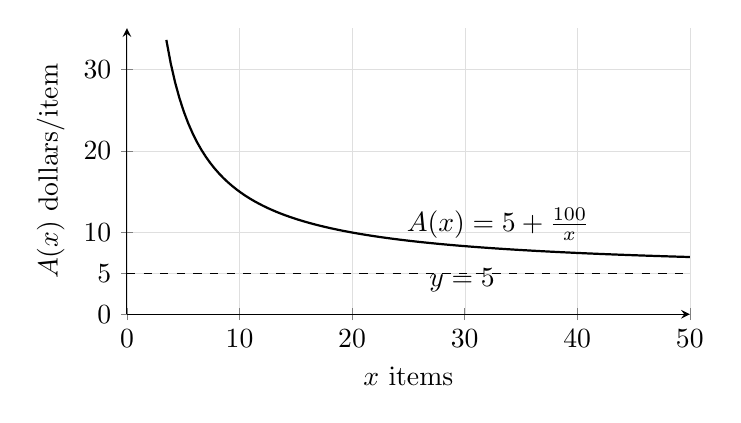
\begin{tikzpicture}
\begin{axis}[
    width=0.72\textwidth,
    height=0.43\textwidth,
    xmin=0, xmax=50,
    ymin=0, ymax=35,
    axis lines=left,
    xlabel={\(x\) items},
    ylabel={\(A(x)\) dollars/item},
    xtick={0,10,20,30,40,50},
    ytick={0,5,10,20,30},
    grid=both,
    grid style={line width=.1pt, draw=gray!25},
]
\addplot[thick, domain=3.5:50, samples=120] {5+100/x};
\addplot[dashed, domain=0:50, samples=2] {5};
\node[anchor=west] at (axis cs:24,11) {\(A(x)=5+\frac{100}{x}\)};
\node[anchor=west] at (axis cs:26,4.1) {\(y=5\)};
\end{axis}
\end{tikzpicture}
\caption{The average cost approaches the variable cost per item as the fixed cost is spread over more items.}
\label{fig:average-cost-asymptote}
\end{figure}

\paragraph{Vertical asymptotes.}
The function

\[
f(x)=\frac{1}{x-2}
\]

is undefined at \(x=2\). As \(x\) gets close to \(2\), the denominator gets close to \(0\), and the quotient grows very large in size.

The vertical line

\[
x=2
\]

is a vertical asymptote.

We will define this precisely with limits. For now, the important picture is this: a rational function can grow without bound near a forbidden input.

\paragraph{A hole instead of an asymptote.}
Not every forbidden input creates an asymptote. Consider

\[
h(x)=\frac{x^2-1}{x-1}.
\]

The input \(x=1\) is forbidden, but for \(x\neq1\),

\[
h(x)=x+1.
\]

So the graph is the line \(y=x+1\) with a hole at the missing point

\[
(1,2).
\]

This is why domain restrictions matter. The formula simplifies, but the missing input remains missing.

\subsection{Algebraic functions}
\label{subsec:algebraic-functions}

Algebraic functions are built from polynomials using a finite number of algebraic operations: addition, subtraction, multiplication, division, and roots.

Examples include

\[
\sqrt{x},
\]

\[
\sqrt{4-x^2},
\]

\[
\frac{\sqrt{x+1}}{x-3},
\]

and

\[
\sqrt[3]{x^2+1}.
\]

These functions often come from geometry.

\paragraph{Example: the upper semicircle.}
The circle of radius \(2\) centered at the origin satisfies

\[
x^2+y^2=4.
\]

Solving for \(y\), we get

\[
y=\pm\sqrt{4-x^2}.
\]

The upper half is

\[
f(x)=\sqrt{4-x^2}.
\]

The square root requires

\[
4-x^2\ge 0.
\]

Thus

\[
-2\le x\le 2.
\]

The natural domain is

\[
[-2,2].
\]

The range is

\[
[0,2].
\]

\paragraph{Example: a root changes smoothness.}
The function

\[
f(x)=\sqrt{x}
\]

has domain

\[
[0,\infty).
\]

Its graph starts at \((0,0)\) and rises slowly after an initially steep beginning. Later, when we study derivatives, we will see that the tangent near \(x=0\) is very different from the tangent of a polynomial.

So algebraic functions can be continuous and natural while still having behavior that needs care.

\subsection{Trigonometric functions in radians}
\label{subsec:trig-functions-radians}

Motion can repeat. A wheel turns. A pendulum swings. A tide rises and falls. A point on a spring oscillates.

The basic functions for periodic motion are sine and cosine.

On the unit circle, an angle \(\theta\) determines a point

\[
(\cos\theta,\sin\theta).
\]

The cosine is the horizontal coordinate. The sine is the vertical coordinate.

\begin{figure}[h]
\centering
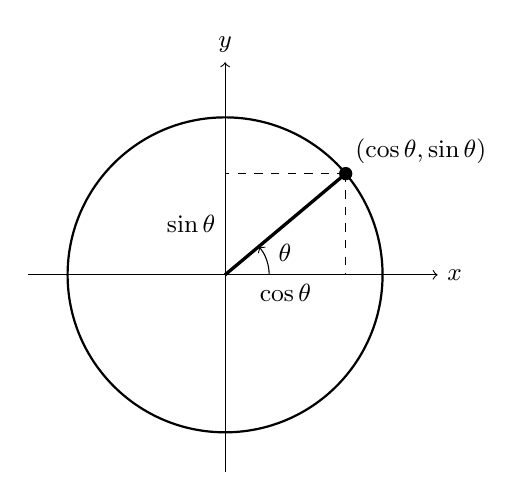
\begin{tikzpicture}[scale=2.0, every node/.style={font=\small}]
  \draw[->] (-1.25,0) -- (1.35,0) node[right] {\(x\)};
  \draw[->] (0,-1.25) -- (0,1.35) node[above] {\(y\)};
  \draw[thick] (0,0) circle (1);

  \def\ang{40}
  \coordinate (P) at ({cos(\ang)},{sin(\ang)});
  \draw[very thick] (0,0) -- (P);
  \draw[dashed] (P) -- ({cos(\ang)},0);
  \draw[dashed] (P) -- (0,{sin(\ang)});
  \fill (P) circle (1.2pt);

  \draw[->] (0.28,0) arc (0:\ang:0.28);
  \node at (0.38,0.14) {\(\theta\)};
  \node[above right] at (P) {\((\cos\theta,\sin\theta)\)};
  \node[below] at ({cos(\ang)/2},0) {\(\cos\theta\)};
  \node[left] at (0,{sin(\ang)/2}) {\(\sin\theta\)};
\end{tikzpicture}
\caption{On the unit circle, cosine and sine are coordinates of the point reached by angle \(\theta\).}
\label{fig:unit-circle-sin-cos}
\end{figure}

The angle must be measured in radians for calculus.

A radian is not an arbitrary unit. It is defined by arc length:

\[
\theta=\frac{\text{arc length}}{\text{radius}}.
\]

On the unit circle, the radius is \(1\), so the radian measure of an angle equals the length of the arc it cuts off.

A full turn has circumference

\[
2\pi,
\]

so a full turn is

\[
2\pi
\]

radians.

A half turn is

\[
\pi
\]

radians.

A quarter turn is

\[
\frac{\pi}{2}
\]

radians.

\begin{quote}
\textbf{Why radians matter.}
The derivative formulas for sine and cosine take their clean form only when angles are measured in radians.

Later we will use the limit

\[
\lim_{h\to0}\frac{\sin h}{h}=1.
\]

That statement is true with \(h\) in radians.
\end{quote}

The sine and cosine functions have domain all real numbers:

\[
\mathbb R.
\]

Their ranges are

\[
[-1,1].
\]

They repeat every \(2\pi\):

\[
\sin(x+2\pi)=\sin x,
\]

\[
\cos(x+2\pi)=\cos x.
\]

The tangent function is

\[
\tan x=\frac{\sin x}{\cos x}.
\]

It is undefined where

\[
\cos x=0.
\]

Thus tangent has vertical asymptotes at

\[
x=\frac{\pi}{2}+k\pi,
\qquad k\in\mathbb Z.
\]

The other trigonometric functions are reciprocals:

\[
\sec x=\frac{1}{\cos x},
\qquad
\csc x=\frac{1}{\sin x},
\qquad
\cot x=\frac{\cos x}{\sin x}.
\]

Their domains must exclude the points where the denominators are zero.

\paragraph{Example: periodic motion.}
A point moving up and down with height

\[
y(t)=3\sin(2t)
\]

has amplitude \(3\), because the output ranges from \(-3\) to \(3\).

The factor \(2\) inside the sine makes the motion repeat faster than \(\sin t\). Since sine repeats when its input increases by \(2\pi\), we need

\[
2t
\]

to increase by \(2\pi\). Therefore \(t\) must increase by \(\pi\). The period is

\[
\pi.
\]

The function

\[
y(t)=3\sin(2t)
\]

repeats every \(\pi\) units of time.

\subsection{Exponential functions}
\label{subsec:exponential-functions}

Linear functions add the same amount for each equal step. Exponential functions multiply by the same factor for each equal step.

A function of the form

\[
f(x)=a^x,
\]

where

\[
a>0,\qquad a\neq1,
\]

is an exponential function.

If \(a>1\), the function grows. If \(0<a<1\), the function decays.

\paragraph{Example: doubling.}
Suppose a bacterial population doubles every \(3\) hours. If the initial population is \(P_0\), then after \(t\) hours a natural model is

\[
P(t)=P_0\,2^{t/3}.
\]

Check the doubling property:

\[
P(t+3)
=
P_0\,2^{(t+3)/3}
=
P_0\,2^{t/3+1}
=
2P_0\,2^{t/3}
=
2P(t).
\]

Every time \(t\) increases by \(3\), the output doubles.

This is the signature of exponential growth: equal time steps produce equal multiplicative changes.

\paragraph{Example: half-life.}
Suppose a radioactive substance loses half its mass every \(8\) days. If the initial mass is \(M_0\), then

\[
M(t)=M_0\left(\frac12\right)^{t/8}.
\]

Then

\[
M(t+8)
=
M_0\left(\frac12\right)^{(t+8)/8}
=
\frac12 M_0\left(\frac12\right)^{t/8}
=
\frac12 M(t).
\]

Every \(8\) days, the mass is cut in half.

\begin{quote}
\textbf{Exponential signature.}
For \(f(x)=a^x\),

\[
f(x+h)=a^{x+h}=a^x a^h.
\]

For a fixed step \(h\), the output is multiplied by the same factor \(a^h\), no matter where the step begins.
\end{quote}

The domain of \(a^x\) is

\[
\mathbb R.
\]

The range is

\[
(0,\infty).
\]

Exponential functions never output \(0\) or a negative number.

One exponential function will become especially important in calculus:

\[
e^x.
\]

The number \(e\) is approximately

\[
2.71828.
\]

Its special role will not be assumed. We will earn it later: \(e^x\) is the exponential function whose rate of change equals itself.

\subsection{Logarithms as inverse functions}
\label{subsec:logarithms-inverse-functions}

Since

\[
a^x
\]

is one-to-one for \(a>0\), \(a\neq1\), it has an inverse. That inverse is the logarithm base \(a\).

\begin{quote}
\textbf{Definition.}
For \(a>0\), \(a\neq1\),

\[
\log_a x=y
\]

means

\[
a^y=x.
\]

In words, \(\log_a x\) is the exponent needed on \(a\) to get \(x\).
\end{quote}

For example,

\[
\log_2 8=3
\]

because

\[
2^3=8.
\]

Also,

\[
\log_{10} 1000=3
\]

because

\[
10^3=1000.
\]

The logarithm has domain

\[
(0,\infty)
\]

and range

\[
\mathbb R.
\]

This is the reverse of the exponential function, whose domain is \(\mathbb R\) and range \((0,\infty)\).

\begin{figure}[h]
\centering
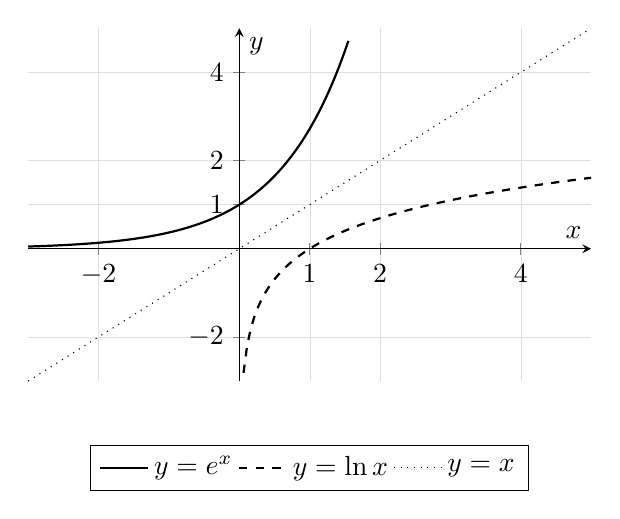
\begin{tikzpicture}
\begin{axis}[
    width=0.72\textwidth,
    height=0.50\textwidth,
    xmin=-3, xmax=5,
    ymin=-3, ymax=5,
    axis lines=middle,
    xlabel={\(x\)},
    ylabel={\(y\)},
    xtick={-2,0,1,2,4},
    ytick={-2,0,1,2,4},
    grid=both,
    grid style={line width=.1pt, draw=gray!25},
    legend style={at={(0.5,-0.18)},anchor=north,legend columns=3}
]
\addplot[thick, domain=-3:1.55, samples=100] {exp(x)};
\addlegendentry{\(y=e^x\)}
\addplot[thick, dashed, domain=0.06:5, samples=100] {ln(x)};
\addlegendentry{\(y=\ln x\)}
\addplot[dotted, domain=-3:5, samples=2] {x};
\addlegendentry{\(y=x\)}
\end{axis}
\end{tikzpicture}
\caption{Exponential and logarithm functions are inverses, so their graphs reflect across the line \(y=x\).}
\label{fig:exp-log-inverses}
\end{figure}

Because logarithms undo exponentials,

\[
\log_a(a^x)=x
\]

for every real \(x\), and

\[
a^{\log_a x}=x
\]

for every \(x>0\).

The exponential laws become logarithm laws. Since

\[
a^u a^v=a^{u+v},
\]

we get

\[
\log_a(xy)=\log_a x+\log_a y,
\qquad x>0,\ y>0.
\]

Since

\[
(a^u)^r=a^{ru},
\]

we get

\[
\log_a(x^r)=r\log_a x,
\qquad x>0.
\]

\paragraph{Example: solving an exponential equation.}
Suppose

\[
2^t=11.
\]

The solution is

\[
t=\log_2 11.
\]

This is already an exact answer. A decimal approximation can be found later, but the logarithm is the number itself.

\paragraph{Natural logarithm.}
The logarithm base \(e\) is called the natural logarithm:

\[
\ln x=\log_e x.
\]

It satisfies

\[
\ln(e^x)=x
\]

and

\[
e^{\ln x}=x,
\qquad x>0.
\]

The word ``natural'' will make more sense after derivatives. For now, remember only that \(e^x\) and \(\ln x\) are inverse functions.

\subsection{The catalog at a glance}
\label{subsec:catalog-glance}

\begin{center}
\renewcommand{\arraystretch}{1.4}
\begin{tabular}{c|c|c|c}
\textbf{family} & \textbf{typical form} & \textbf{natural domain} & \textbf{signature behavior} \\ \hline
linear & \(mx+b\) & \(\mathbb R\) & constant additive change \\
power & \(Cx^p\) & depends on \(p\) & scaling by powers \\
polynomial & \(a_nx^n+\cdots+a_0\) & \(\mathbb R\) & smooth algebraic growth \\
rational & \(\dfrac{p(x)}{q(x)}\) & \(q(x)\neq0\) & ratios, holes, asymptotes \\
algebraic & roots and algebraic operations & depends on roots and denominators & geometric formulas \\
trigonometric & \(\sin x,\cos x,\tan x\) & depends on function & periodic motion \\
exponential & \(a^x\) & \(\mathbb R\) & constant multiplicative change \\
logarithmic & \(\log_a x\) & \((0,\infty)\) & inverse of exponential growth
\end{tabular}
\end{center}

This table is not a substitute for understanding the shapes. It is a map. When a problem mentions constant rate, think linear. When it mentions repeated percentage change, think exponential. When it mentions periodic motion, think trigonometric. When it mentions undoing an exponential, think logarithm.

A function family is a first guess, not a proof. The next step is modeling: choosing a function because units, data, and behavior suggest it. That will be our last preparation before limits turn ``near'' into a precise mathematical tool.
\section{Models before calculus}
\label{sec:models-before-calculus}

The catalog gave us familiar function families. A model is the next step: we choose one of those families because a situation asks for it.

A model is not the same thing as reality. It is a mathematical story about reality. A good model respects units, captures the main pattern, and makes predictions we can test.

\begin{quote}
\textbf{Definition.}
A \emph{mathematical model} is a function, equation, graph, or table used to represent a real quantity.

A model should be judged by four questions:

\[
\text{What assumptions does it make?}
\]

\[
\text{Do the units make sense?}
\]

\[
\text{How well does it fit the information we have?}
\]

\[
\text{Where should we not trust it?}
\]
\end{quote}

Calculus will later tell us how models change and how their effects accumulate. Before calculus begins, we should learn the main shapes that models can take.

\subsection{Linear growth}
\label{subsec:linear-growth-models}

Suppose water is poured into a tank at a steady rate of \(3\) liters per minute. At the moment we start watching, the tank already contains \(12\) liters.

After \(t\) minutes, the amount of water is

\[
W(t)=12+3t.
\]

The number \(12\) is the starting amount. The number \(3\) is the rate of change.

\[
\begin{array}{c|ccccc}
t\text{ (minutes)} & 0 & 1 & 2 & 3 & 4 \\ \hline
W(t)\text{ (liters)} & 12 & 15 & 18 & 21 & 24
\end{array}
\]

Each time \(t\) increases by \(1\), the output increases by \(3\).

\[
15-12=3,\qquad 18-15=3,\qquad 21-18=3.
\]

This is the signature of a linear model: equal input changes produce equal output changes.

\begin{quote}
\textbf{Linear model.}
A linear model has the form

\[
y=b+mx.
\]

The number \(b\) is the initial value, because

\[
y(0)=b.
\]

The number \(m\) is the constant rate of change:

\[
m=\frac{\text{change in output}}{\text{change in input}}.
\]
\end{quote}

The units of \(m\) are output units divided by input units. In the water example,

\[
m=3\frac{\text{liters}}{\text{minute}}.
\]

So

\[
3\frac{\text{liters}}{\text{minute}}\cdot t\text{ minutes}
=
3t\text{ liters}.
\]

The units are not decoration. They check the formula.

\paragraph{Example: a phone plan.}
A phone plan charges \(25\) dollars per month plus \(0.05\) dollars per text message. If \(n\) is the number of text messages, the monthly cost is

\[
C(n)=25+0.05n.
\]

The slope is

\[
0.05\frac{\text{dollars}}{\text{message}}.
\]

The intercept is

\[
25\text{ dollars}.
\]

The natural domain is

\[
n=0,1,2,3,\ldots,
\]

because the number of text messages must be a whole number. The graph is a collection of points, not a solid line. We often draw the line anyway because it makes the pattern easy to see, but the model's meaning decides the real domain.

\paragraph{Finding a linear model from two points.}
Suppose a candle has height \(18\) cm at time \(t=0\), and height \(14\) cm after \(2\) hours. If we assume the candle burns at a constant rate, then its height is linear.

The slope is

\[
m=
\frac{14-18}{2-0}
=
\frac{-4}{2}
=
-2
\]

cm/hour. Therefore

\[
H(t)=18-2t.
\]

This model predicts that the candle reaches height \(0\) when

\[
18-2t=0.
\]

So

\[
t=9.
\]

The model says the candle lasts \(9\) hours.

But this prediction depends on the assumption that the burn rate stays constant. If the candle shape changes or the flame weakens, the model may fail before \(9\) hours.

\begin{quote}
\textbf{Modeling lesson.}
A formula can be algebraically correct and still be physically wrong outside the range where its assumptions make sense.
\end{quote}

\subsection{Power-law scaling}
\label{subsec:power-law-models}

Linear models are about constant additive change. Power-law models are about scaling.

Imagine enlarging a square photograph. If every length is multiplied by \(2\), then the area is multiplied by \(4\).

A \(3\)-inch by \(3\)-inch square has area

\[
9\text{ square inches}.
\]

A \(6\)-inch by \(6\)-inch square has area

\[
36\text{ square inches}.
\]

Doubling the side length quadruples the area:

\[
36=4\cdot 9.
\]

This is not linear growth. It is square growth.

For a square of side length \(s\), the area is

\[
A(s)=s^2.
\]

If we multiply the side length by \(k\), then

\[
A(ks)=(ks)^2=k^2s^2=k^2A(s).
\]

So scaling the input by \(k\) scales the output by \(k^2\).

\begin{quote}
\textbf{Power-law model.}
A power-law model has the form

\[
y=Cx^p,
\]

where \(C\) and \(p\) are constants.

It satisfies the scaling rule

\[
y(kx)=C(kx)^p=k^pCx^p=k^p y(x).
\]
\end{quote}

The exponent \(p\) tells us how strongly the output responds to scaling.

\[
\begin{array}{c|c|c}
\textbf{model} & \textbf{doubling input multiplies output by} & \textbf{common meaning} \\ \hline
y=Cx & 2 & \text{length-like growth} \\
y=Cx^2 & 4 & \text{area-like growth} \\
y=Cx^3 & 8 & \text{volume-like growth} \\
y=C\sqrt{x}=Cx^{1/2} & \sqrt2 & \text{root-type growth}
\end{array}
\]

\paragraph{Example: similar tanks.}
Suppose two water tanks have the same shape, but one is twice as tall, twice as wide, and twice as deep as the other.

Every length has been multiplied by \(2\). Volume is three-dimensional, so the larger tank has

\[
2^3=8
\]

times the volume.

If a tank of height \(h\) has volume

\[
V(h)=Ch^3
\]

for some constant \(C\), then

\[
V(2h)=C(2h)^3=8Ch^3=8V(h).
\]

This is why a small-looking change in length can make a large change in volume.

\paragraph{Example: units suggest a power.}
Suppose a quantity depends only on a length \(r\), and the output has units of area. Since area units are length squared, a first guess is

\[
A(r)=Cr^2.
\]

For a circle, the constant is

\[
C=\pi,
\]

so

\[
A(r)=\pi r^2.
\]

If the output has units of volume, a first guess is

\[
V(r)=Cr^3.
\]

For a sphere, the constant is

\[
C=\frac43\pi,
\]

so

\[
V(r)=\frac43\pi r^3.
\]

Units do not prove the formula. But they often tell us what kind of formula to expect.

\subsection{Exponential growth and decay}
\label{subsec:exponential-models}

Some quantities do not add the same amount in equal time steps. They multiply by the same factor.

Suppose a bacterial culture grows by \(50\%\) every hour. If it starts with \(100\) bacteria, then after each hour the population is multiplied by \(1.5\).

\[
\begin{array}{c|ccccc}
t\text{ (hours)} & 0 & 1 & 2 & 3 & 4 \\ \hline
P(t) & 100 & 150 & 225 & 337.5 & 506.25
\end{array}
\]

The differences are not constant:

\[
150-100=50,
\]

\[
225-150=75,
\]

\[
337.5-225=112.5.
\]

But the ratios are constant:

\[
\frac{150}{100}=1.5,
\qquad
\frac{225}{150}=1.5,
\qquad
\frac{337.5}{225}=1.5.
\]

This is exponential growth.

The model is

\[
P(t)=100(1.5)^t.
\]

\begin{quote}
\textbf{Exponential model.}
An exponential model has the form

\[
y=Aa^t,
\]

where

\[
A>0,\qquad a>0.
\]

The number \(A\) is the initial value. The number \(a\) is the growth factor per unit time.

If \(a>1\), the model grows.

If \(0<a<1\), the model decays.
\end{quote}

\paragraph{Example: half-life.}
A substance has half-life \(8\) days. That means its amount is multiplied by \(\frac12\) every \(8\) days.

If the starting amount is \(M_0\), then a model for the amount after \(t\) days is

\[
M(t)=M_0\left(\frac12\right)^{t/8}.
\]

Check the half-life property:

\[
M(t+8)
=
M_0\left(\frac12\right)^{(t+8)/8}
=
M_0\left(\frac12\right)^{t/8+1}
=
\frac12 M_0\left(\frac12\right)^{t/8}
=
\frac12 M(t).
\]

Every \(8\) days, the amount is cut in half.

\paragraph{Example: doubling time.}
A population doubles every \(5\) years. If the initial population is \(P_0\), then

\[
P(t)=P_0\,2^{t/5}.
\]

Indeed,

\[
P(t+5)
=
P_0\,2^{(t+5)/5}
=
P_0\,2^{t/5+1}
=
2P(t).
\]

The exponent

\[
\frac{t}{5}
\]

counts how many doubling periods have passed.

\begin{figure}[h]
\centering
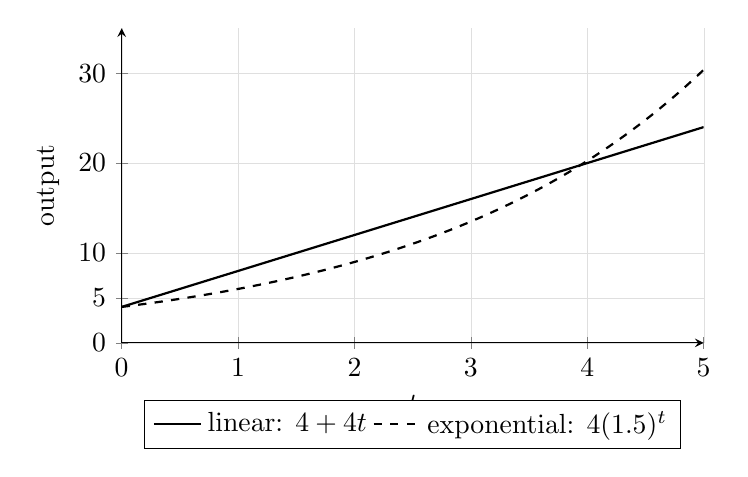
\begin{tikzpicture}
\begin{axis}[
    width=0.74\textwidth,
    height=0.46\textwidth,
    xmin=0, xmax=5,
    ymin=0, ymax=35,
    axis lines=left,
    xlabel={\(t\)},
    ylabel={output},
    xtick={0,1,2,3,4,5},
    ytick={0,5,10,20,30},
    grid=both,
    grid style={line width=.1pt, draw=gray!25},
    legend style={at={(0.5,-0.18)},anchor=north,legend columns=2}
]
\addplot[thick, domain=0:5, samples=2] {4+4*x};
\addlegendentry{linear: \(4+4t\)}
\addplot[thick, dashed, domain=0:5, samples=100] {4*1.5^x};
\addlegendentry{exponential: \(4(1.5)^t\)}
\end{axis}
\end{tikzpicture}
\caption{Linear growth adds equal amounts. Exponential growth multiplies by equal factors.}
\label{fig:linear-versus-exponential-models}
\end{figure}

\paragraph{A warning.}
Exponential growth can be a good short-term model and a terrible long-term model.

A bacterial population cannot grow forever in a closed dish. A rumor cannot spread to more people than exist. A bank account cannot earn the same interest rate through every possible economic condition.

A model may be useful because it is locally accurate, even when it is not globally permanent. Calculus will often help us decide what ``locally'' means.

\subsection{Periodic motion}
\label{subsec:periodic-motion-models}

Some quantities repeat.

A Ferris wheel turns. A tide rises and falls. A weight on a spring moves up and down. A point on a rotating tire returns to its starting height again and again.

The basic models for repeating motion use sine and cosine.

\paragraph{Example: height on a Ferris wheel.}
Suppose a Ferris wheel has center \(20\) meters above the ground and radius \(18\) meters. One full rotation takes \(30\) seconds.

If a rider starts at the midline and is moving upward at time \(t=0\), then the height can be modeled by

\[
H(t)=20+18\sin\left(\frac{\pi t}{15}\right).
\]

The number \(20\) is the midline. The number \(18\) is the amplitude. The period is \(30\), because

\[
\sin\left(\frac{\pi(t+30)}{15}\right)
=
\sin\left(\frac{\pi t}{15}+2\pi\right)
=
\sin\left(\frac{\pi t}{15}\right).
\]

So

\[
H(t+30)=H(t).
\]

The height repeats every \(30\) seconds.

\begin{figure}[h]
\centering
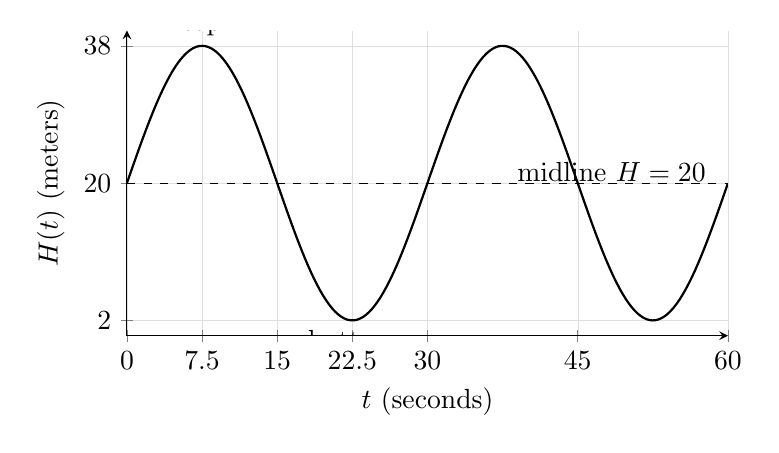
\begin{tikzpicture}
\begin{axis}[
    width=0.76\textwidth,
    height=0.45\textwidth,
    xmin=0, xmax=60,
    ymin=0, ymax=40,
    axis lines=left,
    xlabel={\(t\) (seconds)},
    ylabel={\(H(t)\) (meters)},
    xtick={0,7.5,15,22.5,30,45,60},
    xticklabels={\(0\),\(7.5\),\(15\),\(22.5\),\(30\),\(45\),\(60\)},
    ytick={2,20,38},
    yticklabels={\(2\),\(20\),\(38\)},
    grid=both,
    grid style={line width=.1pt, draw=gray!25},
]
\addplot[thick, domain=0:60, samples=200] {20+18*sin(deg(pi*x/15))};
\addplot[dashed, domain=0:60, samples=2] {20};
\node[anchor=west] at (axis cs:38,21.5) {midline \(H=20\)};
\node[anchor=south] at (axis cs:7.5,38) {top};
\node[anchor=north] at (axis cs:22.5,2) {bottom};
\end{axis}
\end{tikzpicture}
\caption{A sinusoidal model records a repeating motion by its midline, amplitude, and period.}
\label{fig:ferris-wheel-model}
\end{figure}

\begin{quote}
\textbf{Periodic model.}
A function is \emph{periodic} if there is a positive number \(T\) such that

\[
f(t+T)=f(t)
\]

for every allowed \(t\).

The smallest such positive \(T\), when it exists, is called the \emph{period}.
\end{quote}

For

\[
A\sin(Bt)
\]

and

\[
A\cos(Bt),
\]

the amplitude is

\[
|A|,
\]

and the period is

\[
\frac{2\pi}{B},
\qquad B>0.
\]

\paragraph{Example.}
The function

\[
y(t)=5\cos(4t)
\]

has amplitude

\[
5
\]

and period

\[
\frac{2\pi}{4}=\frac{\pi}{2}.
\]

The output repeats whenever \(t\) increases by \(\frac{\pi}{2}\).

\subsection{Choosing a model from units and data}
\label{subsec:choosing-model-units-data}

A model is a choice. The choice should be guided by the situation.

\begin{tabular}{c|>{\centering\arraybackslash}p{3.5cm}|>{\centering\arraybackslash}p{4cm}|>{\centering\arraybackslash}p{4.5cm}}
\textbf{family} & \textbf{typical form} & \textbf{natural domain} & \textbf{signature behavior} \\ \hline
linear & \(mx+b\) & \(\mathbb R\) & constant additive change \\
power & \(Cx^p\) & depends on \(p\) & scaling by powers \\
polynomial & \(a_nx^n+\cdots+a_0\) & \(\mathbb R\) & smooth algebraic growth \\
rational & \(\dfrac{p(x)}{q(x)}\) & \(q(x)\neq0\) & ratios, holes, asymptotes \\
algebraic & roots and algebraic operations & depends on roots and denominators & geometric formulas \\
trigonometric & \(\sin x,\cos x,\tan x\) & depends on function & periodic motion \\
exponential & \(a^x\) & \(\mathbb R\) & constant multiplicative change \\
logarithmic & \(\log_a x\) & \((0,\infty)\) & inverse of exponential growth
\end{tabular}

\paragraph{Example: linear or exponential?}
A small plant is measured once per week.

\[
\begin{array}{c|ccccc}
t\text{ (weeks)} & 0 & 1 & 2 & 3 & 4 \\ \hline
H(t)\text{ (cm)} & 10 & 13 & 16 & 19 & 22
\end{array}
\]

The differences are

\[
3,\quad 3,\quad 3,\quad 3.
\]

A linear model is natural:

\[
H(t)=10+3t.
\]

Now compare a different table:

\[
\begin{array}{c|ccccc}
t\text{ (hours)} & 0 & 1 & 2 & 3 & 4 \\ \hline
P(t) & 100 & 150 & 224 & 337 & 506
\end{array}
\]

The differences are

\[
50,\quad 74,\quad 113,\quad 169,
\]

not constant. But the ratios are approximately

\[
1.50,\quad 1.49,\quad 1.50,\quad 1.50.
\]

An exponential model is natural:

\[
P(t)\approx 100(1.5)^t.
\]

The symbol \(\approx\) matters. Data are often measured with error, and real processes rarely follow a model perfectly.

\paragraph{Residuals: the errors a model leaves behind.}
Suppose data points are

\[
(x_1,y_1),\quad (x_2,y_2),\quad \ldots,\quad (x_n,y_n),
\]

and a model predicts

\[
y=f(x).
\]

At input \(x_i\), the prediction error is

\[
y_i-f(x_i).
\]

These errors are called \emph{residuals}. A good model should leave small residuals without using a formula that is more complicated than the situation deserves.

\begin{quote}
\textbf{A modeling habit.}
Do not ask only:

\[
\text{Can I find a formula through the data?}
\]

Ask also:

\[
\text{Does the formula explain the pattern?}
\]

\[
\text{Are the units meaningful?}
\]

\[
\text{Does the formula behave reasonably outside the data?}
\]
\end{quote}

\paragraph{Example: a model that fits too well.}
Given five data points, it is often possible to find a polynomial of degree \(4\) that passes exactly through all of them. That does not mean the polynomial is the best model.

A high-degree polynomial may wiggle wildly between data points or make absurd predictions just outside the measured interval. Exact fit is not the same as understanding.

For calculus, the simplest useful model is often better than a complicated perfect fit.

Models give us functions to study. Technology gives us quick graphs of those functions. But a graph on a screen is not the function itself. It is a picture made with choices: a window, a scale, and a finite number of sampled points.

Those choices can hide the truth.

\section{Technology and graphs}
\label{sec:technology-and-graphs}

A graphing calculator or computer can draw in a second what would take minutes by hand. That speed is useful. It is also dangerous.

A screen does not show a function. It shows a sampled picture of a function in a chosen window.

The picture may be excellent. It may also miss a hole, hide a turn, smooth out an oscillation, or round away a small but important difference.

The right attitude is not distrust. It is partnership.

\begin{quote}
\textbf{Use technology to see. Use mathematics to check.}
\end{quote}

\subsection{Windows can lie}
\label{subsec:windows-can-lie}

A graphing window is a rectangle:

\[
x_{\min}\le x\le x_{\max},
\qquad
y_{\min}\le y\le y_{\max}.
\]

Anything outside that rectangle is invisible. The same function can look simple in one window and complicated in another.

\paragraph{Example.}
Consider

\[
p(x)=x^3-6x.
\]

Near the origin, in the small window

\[
-1\le x\le 1,
\]

the graph looks like a steep decreasing curve. But in the wider window

\[
-3\le x\le 3,
\]

we see more of its shape: it rises, falls, and rises again.

\begin{figure}[h]
\centering
\begin{minipage}{0.47\textwidth}
\centering
\begin{tikzpicture}
\begin{axis}[
    width=\textwidth,
    height=0.76\textwidth,
    xmin=-1, xmax=1,
    ymin=-6, ymax=6,
    axis lines=middle,
    xlabel={\(x\)},
    ylabel={\(y\)},
    xtick={-1,0,1},
    ytick={-6,0,6},
    grid=both,
    grid style={line width=.1pt, draw=gray!25},
    title={small window}
]
\addplot[thick, domain=-1:1, samples=100] {x^3-6*x};
\end{axis}
\end{tikzpicture}
\end{minipage}
\hfill
\begin{minipage}{0.47\textwidth}
\centering
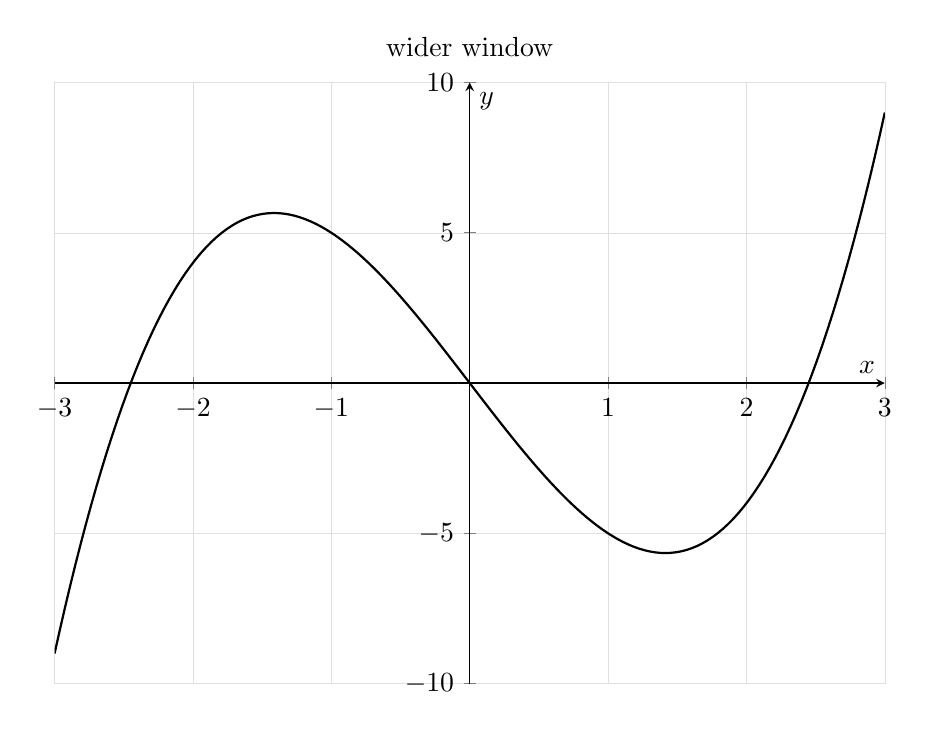
\begin{tikzpicture}
\begin{axis}[
    width=\textwidth,
    height=0.76\textwidth,
    xmin=-3, xmax=3,
    ymin=-10, ymax=10,
    axis lines=middle,
    xlabel={\(x\)},
    ylabel={\(y\)},
    xtick={-3,-2,-1,0,1,2,3},
    ytick={-10,-5,0,5,10},
    grid=both,
    grid style={line width=.1pt, draw=gray!25},
    title={wider window}
]
\addplot[thick, domain=-3:3, samples=160] {x^3-6*x};
\end{axis}
\end{tikzpicture}
\end{minipage}
\caption{The small window is not false; it is incomplete. A wider window reveals behavior the first picture cannot show.}
\label{fig:window-can-lie-cubic}
\end{figure}

The function did not change. The window changed.

\paragraph{Example: a hidden hole.}
The function

\[
h(x)=\frac{x^2-1}{x-1}
\]

is not defined at

\[
x=1.
\]

For \(x\neq1\), it simplifies:

\[
h(x)=\frac{(x-1)(x+1)}{x-1}=x+1.
\]

A graphing utility may draw the line

\[
y=x+1
\]

without showing the missing point. But the original function has a hole at

\[
(1,2).
\]

The screen may not show the difference between

\[
h(x)=\frac{x^2-1}{x-1}
\]

and

\[
\ell(x)=x+1.
\]

Algebra does.

\begin{quote}
\textbf{Window warning.}
A graph can suggest:

\[
\text{There may be a zero, a turn, a hole, or an asymptote.}
\]

It cannot by itself prove:

\[
\text{There is exactly one, or none, or always.}
\]
\end{quote}

\subsection{Sampling can miss behavior}
\label{subsec:sampling-can-miss-behavior}

A computer cannot check infinitely many points. It samples finitely many input values, plots the corresponding output values, and connects or displays them.

Usually this works well. Sometimes it fails spectacularly.

\paragraph{Example: the zero-looking oscillation.}
Consider

\[
f(x)=\sin(100\pi x),
\qquad 0\le x\le 1.
\]

This function oscillates \(50\) full times on the interval \([0,1]\).

But if a graphing program happens to sample at

\[
x=0,\ 0.01,\ 0.02,\ \ldots,\ 1.00,
\]

then every sampled value is

\[
\sin(100\pi x)=0.
\]

For example,

\[
\sin(100\pi\cdot 0.37)=\sin(37\pi)=0.
\]

The sampled graph may look like the horizontal line \(y=0\), even though the true function swings from \(-1\) to \(1\) again and again between the sampled points.

\begin{figure}[h]
\centering
\begin{minipage}{0.47\textwidth}
\centering
\begin{tikzpicture}
\begin{axis}[
    width=\textwidth,
    height=0.74\textwidth,
    xmin=0, xmax=1,
    ymin=-1.2, ymax=1.2,
    axis lines=middle,
    xlabel={\(x\)},
    ylabel={\(y\)},
    xtick={0,0.5,1},
    ytick={-1,0,1},
    grid=both,
    grid style={line width=.1pt, draw=gray!25},
    title={poor sampling}
]
\addplot[thick, domain=0:1, samples=101] {sin(deg(100*pi*x))};
\addplot[only marks, mark=*, mark size=0.45pt, domain=0:1, samples=101] {sin(deg(100*pi*x))};
\end{axis}
\end{tikzpicture}
\end{minipage}
\hfill
\begin{minipage}{0.47\textwidth}
\centering
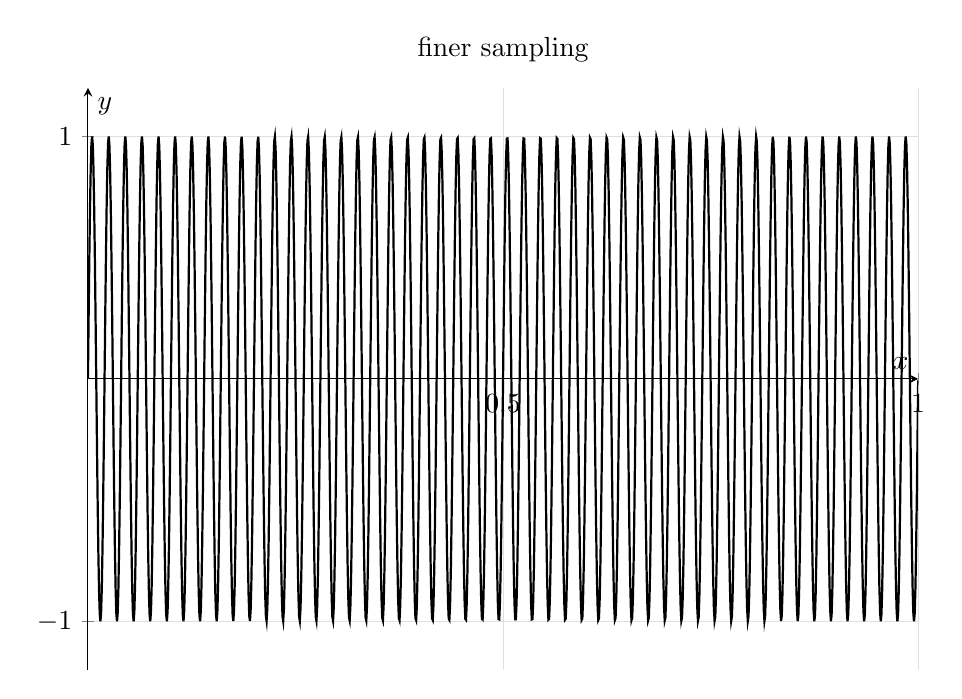
\begin{tikzpicture}
\begin{axis}[
    width=\textwidth,
    height=0.74\textwidth,
    xmin=0, xmax=1,
    ymin=-1.2, ymax=1.2,
    axis lines=middle,
    xlabel={\(x\)},
    ylabel={\(y\)},
    xtick={0,0.5,1},
    ytick={-1,0,1},
    grid=both,
    grid style={line width=.1pt, draw=gray!25},
    title={finer sampling}
]
\addplot[thick, domain=0:1, samples=1200] {sin(deg(100*pi*x))};
\end{axis}
\end{tikzpicture}
\end{minipage}
\caption{A finite sample can miss oscillation. The left picture suggests \(f(x)=0\). The right picture shows the hidden motion.}
\label{fig:sampling-misses-oscillation}
\end{figure}

 Oscillations appear in sound, light, vibration, and signal processing. Sampling matters.

\begin{quote}
\textbf{Sampling warning.}
A graph drawn from samples is trustworthy only at the scale the sampling can see.
\end{quote}

\subsection{Numerical evidence versus proof}
\label{subsec:numerical-evidence-versus-proof}

Numerical evidence is useful. It helps us guess patterns. It helps us find examples. It helps us notice mistakes.

But a long list of checked cases is not a proof.

\paragraph{Example: a graph suggests positivity.}
The graph of

\[
q(x)=x^2-2x+2
\]

appears to lie above the \(x\)-axis. That suggests

\[
q(x)>0
\]

for all real \(x\).

A graph supports the claim, but algebra proves it:

\[
x^2-2x+2
=
(x-1)^2+1.
\]

Since

\[
(x-1)^2\ge0,
\]

we have

\[
(x-1)^2+1\ge1.
\]

Therefore

\[
q(x)\ge1>0
\]

for every real \(x\).

The proof tells us more than the graph. It tells us that the function is not merely positive; it is at least \(1\).

\paragraph{Example: a sign change suggests a root.}
Consider

\[
r(x)=x^3-x-1.
\]

We can compute

\[
r(1)=1-1-1=-1
\]

and

\[
r(2)=8-2-1=5.
\]

The outputs change from negative to positive between \(x=1\) and \(x=2\). A graph suggests that the curve crosses the \(x\)-axis somewhere between them.

Later, after we define continuity, the Intermediate Value Theorem will make this exact. It will say that a continuous function that changes sign on an interval must have a zero inside that interval.

For now, the important lesson is this:

\[
\text{numerical evidence gives a clue;}
\]

\[
\text{a theorem explains when the clue is reliable.}
\]

\paragraph{Example: many correct cases do not prove an identity.}
Suppose a calculator suggests that two formulas give the same output for many inputs. That does not prove the formulas are identical.

For example, the functions

\[
f(x)=x^2
\]

and

\[
g(x)=x^2+(x-1)(x-2)(x-3)(x-4)(x-5)
\]

agree at

\[
x=1,2,3,4,5.
\]

At each of those inputs, the product term is \(0\), so

\[
g(x)=x^2.
\]

But the functions are not the same. At \(x=0\),

\[
f(0)=0,
\]

while

\[
g(0)=0+(-1)(-2)(-3)(-4)(-5)=-120.
\]

Checking five points was not enough. Checking a thousand points is still not a proof of equality for all real numbers.

\begin{quote}
\textbf{Proof warning.}
A computation can show that a statement is true at the inputs tested.

A proof shows why the statement must be true for every allowed input.
\end{quote}

\subsection{A first warning about roundoff}
\label{subsec:first-warning-roundoff}

There is another way technology can mislead: numbers are rounded.

A calculator screen may show \(10\) digits. A computer may store more. But still, it stores only finitely many digits. Most real numbers cannot be stored exactly.

Usually this causes no visible trouble. But when two nearly equal numbers are subtracted, important digits can disappear.

\paragraph{Example: subtracting nearly equal numbers.}
Consider

\[
Q(h)=\frac{\sqrt{1+h}-1}{h}.
\]

This expression will appear naturally when we study the derivative of \(\sqrt{x}\). For small \(h\), the numerator

\[
\sqrt{1+h}-1
\]

subtracts two numbers very close to each other.

If \(h=10^{-12}\), then

\[
\sqrt{1+h}
\]

is extremely close to \(1\). A rounded calculation may lose the small difference.

But algebra gives a safer expression. Multiply numerator and denominator by the conjugate:

\[
Q(h)
=
\frac{\sqrt{1+h}-1}{h}
\cdot
\frac{\sqrt{1+h}+1}{\sqrt{1+h}+1}.
\]

Then

\[
Q(h)
=
\frac{(1+h)-1}{h(\sqrt{1+h}+1)}
=
\frac{h}{h(\sqrt{1+h}+1)}.
\]

For \(h\neq0\),

\[
Q(h)=\frac{1}{\sqrt{1+h}+1}.
\]

Now there is no subtraction of nearly equal numbers.

As \(h\) becomes small, this safer expression is close to

\[
\frac{1}{1+1}=\frac12.
\]

\begin{quote}
\textbf{Roundoff warning.}
Two algebraically equal formulas can behave differently when approximately computed on a calculator.

The problem is not the mathematics. The problem is the finite storage of decimal or binary approximations.
\end{quote}

\paragraph{Why this matters for calculus.}
Calculus is built from small changes:

\[
\frac{f(a+h)-f(a)}{h}.
\]

When \(h\) is very small, the numerator often subtracts nearly equal numbers. That makes roundoff error part of the story.

This does not mean we should avoid numerical computation. It means we should understand what the computation is doing.

Sometimes, algebra can make a formula more (numerically) stable. Sometimes a graph needs a better range for variables. Sometimes, a numerical pattern needs a precise definition.

The next chapter provides the missing language. It will make the phrase

\[
\text{as }x\text{ gets close to }a
\]

into mathematics. That language is the limit.
\section{Chapter review and discovery problems}
\label{sec:chapter-2-review}

Chapter 1 began with motion. It asked how to pass between velocity and distance, slope and area, difference and sum.

Chapter 2 built the language that this question needs. We used the real line to measure nearness, functions to record dependence, graphs to see geometric behavior, and models to connect formulas with real applications. We also learned that a graph on a screen is only evidence, not proof.

The next chapter returns to the original motion problem. But now we are ready to say what ``near'' means.

\subsection{Chapter map}
\label{subsec:chapter-2-map}

\begin{center}
\renewcommand{\arraystretch}{1.35}
\begin{tabular}{p{0.23\textwidth}|p{0.34\textwidth}|p{0.34\textwidth}}
\textbf{idea} & \textbf{what it means} & \textbf{why calculus needs it} \\ \hline
real line & numbers as points and distances & limits need a precise language of closeness \\ \hline
intervals & unbroken pieces of the real line & inputs often live on intervals \\ \hline
absolute value & distance from \(0\), or distance between two numbers & error is measured by inequalities such as \(|A-T|<\varepsilon\) \\ \hline
completeness & the real line has no gaps & limiting processes should have destinations \\ \hline
function & one allowed output for each allowed input & calculus studies how outputs change when inputs change \\ \hline
domain & the allowed inputs & derivative and limit questions must respect where a function is defined \\ \hline
graph & a picture of all input-output pairs & slope, sign, roots, and behavior become visible \\ \hline
composition & one function feeds another & the chain rule will come from this structure \\ \hline
inverse function & a function that undoes another & logarithms, inverse trigonometric functions, and inverse rates depend on this idea \\ \hline
model & a function chosen to represent a situation & calculus measures change and accumulation in models
\end{tabular}
\end{center}

\subsection{Concept check: function versus formula}
\label{subsec:concept-check-function-formula}

Answer these without a calculator unless a problem explicitly asks for one. Use complete sentences when the question asks for an explanation.

\begin{enumerate}
\item Explain the difference between the intervals

\[
(2,5),\qquad [2,5],\qquad [2,5).
\]

Which endpoints are included in each?

\item Why do we never write

\[
[2,\infty]
\]

as an interval?

\item Explain why

\[
|x-a|<\varepsilon
\]

means that \(x\) is within distance \(\varepsilon\) of \(a\).

\item Write

\[
|x-7|<0.01
\]

as a double inequality.

\item Explain why the formula

\[
f(x)=x^2
\]

does not completely describe a function until the domain is known.

\item Give two different functions that use the same formula

\[
x^2
\]

but have different ranges.

\item A table gives the temperature of a cup of tea at times

\[
0,1,2,3,4.
\]

Does the table automatically define the temperature at \(t=2.5\)? Explain.

\item The equation

\[
x^2+y^2=1
\]

does not define \(y\) as a function of \(x\) on \([-1,1]\). Explain why.

\item The upper semicircle

\[
y=\sqrt{1-x^2}
\]

does define \(y\) as a function of \(x\). What is its domain? What is its range?

\item Explain why

\[
h(x)=\frac{x^2-1}{x-1}
\]

is not the same function as

\[
p(x)=x+1
\]

when \(p\) has domain \(\mathbb R\).

\item What does the vertical line test check?

\item What does the horizontal line test check?

\item Explain why \(f^{-1}(x)\) usually does not mean

\[
\frac{1}{f(x)}.
\]

\item Suppose

\[
f(3)=10.
\]

What point is on the graph of \(f\)? If \(f\) has an inverse, what corresponding point is on the graph of \(f^{-1}\)?

\item Why does order matter in a composition such as

\[
f(g(x))?
\]

\item Why are radians the natural angle measure for calculus?

\item A graphing utility shows that a function appears positive in the window

\[
-10\le x\le 10.
\]

Does that prove the function is positive for all real \(x\)? Explain.

\item What is a residual in a modeling problem?

\item A model fits five measured data points exactly. Why might it still be a poor model?

\item The rational numbers contain fractions between any two fractions. Why does that fact alone not make the rational number line complete?
\end{enumerate}

\subsection{Skills: intervals, domains, transformations, and inverses}
\label{subsec:skills-domains-transformations}

\paragraph{Intervals and absolute value.}
Solve each inequality and write the answer in interval notation.

\begin{enumerate}
\item

\[
-3<x\le 4.
\]

\item

\[
|x-2|<5.
\]

\item

\[
|x+1|\le 3.
\]

\item

\[
|2x-5|<1.
\]

\item

\[
x^2<16.
\]

\item

\[
x^2\ge 9.
\]

\item

\[
\frac{1}{x-4}
\]

is defined.

\item

\[
\sqrt{2x+6}
\]

is defined.

\item

\[
\sqrt{9-x^2}
\]

is defined.

\item

\[
\ln(x-5)
\]

is defined.
\end{enumerate}

\paragraph{Natural domains.}
Find the natural domain of each function.

\begin{enumerate}
\item

\[
f(x)=\sqrt{x-3}.
\]

\item

\[
g(x)=\frac{1}{x^2-9}.
\]

\item

\[
h(x)=\frac{\sqrt{x+2}}{x-1}.
\]

\item

\[
p(x)=\sqrt{16-x^2}.
\]

\item

\[
q(x)=\frac{1}{\sqrt{x+4}}.
\]

\item

\[
r(x)=\ln(7-2x).
\]

\item

\[
s(x)=\sqrt{x^2-1}.
\]

\item

\[
u(x)=\frac{\ln x}{x-3}.
\]
\end{enumerate}

\paragraph{Ranges.}
Find the range of each function on the stated domain.

\begin{enumerate}
\item

\[
f(x)=x^2,\qquad -2\le x\le 3.
\]

\item

\[
g(x)=x^2,\qquad 0\le x\le 3.
\]

\item

\[
h(x)=\sqrt{x},\qquad 0\le x\le 9.
\]

\item

\[
p(x)=4-x^2,\qquad -1\le x\le 2.
\]

\item

\[
q(x)=2+\sin x,\qquad x\in\mathbb R.
\]
\end{enumerate}

\paragraph{Graph transformations.}
Let \(y=f(x)\) be a function with domain \([-2,4]\) and range \([-1,3]\). For each new function, describe the graph transformation and find the new domain and range.

\begin{enumerate}
\item

\[
g(x)=f(x)+5.
\]

\item

\[
h(x)=f(x-3).
\]

\item

\[
p(x)=f(x+2).
\]

\item

\[
q(x)=-f(x).
\]

\item

\[
r(x)=2f(x).
\]

\item

\[
s(x)=f(2x).
\]

\item

\[
u(x)=f\left(\frac{x}{2}\right).
\]

\item

\[
v(x)=3-f(x-1).
\]
\end{enumerate}

\paragraph{Composition.}
Let

\[
f(x)=\sqrt{x},
\qquad
g(x)=4-x^2,
\qquad
r(x)=\frac{1}{x-1}.
\]

For each expression, find the formula and the domain.

\begin{enumerate}
\item

\[
(f\circ g)(x).
\]

\item

\[
(g\circ f)(x).
\]

\item

\[
(r\circ f)(x).
\]

\item

\[
(f\circ r)(x).
\]

\item

\[
(g\circ r)(x).
\]

\item

\[
(r\circ g)(x).
\]
\end{enumerate}

\paragraph{Inverse functions.}
Find the inverse function, including its domain and range.

\begin{enumerate}
\item

\[
f(x)=3x-7.
\]

\item

\[
g(x)=\frac{x+1}{2}.
\]

\item

\[
h(x)=x^2,\qquad x\ge 0.
\]

\item

\[
p(x)=x^2,\qquad x\le 0.
\]

\item

\[
q(x)=\frac{x-2}{x+1},\qquad x\neq -1.
\]

\item

\[
r(x)=e^{x-4}.
\]
\end{enumerate}

\subsection{Skills: reading a graph}
\label{subsec:skills-reading-graph}

The graph below shows

\[
p(x)=\frac{1}{10}(x+3)(x-1)(x-4).
\]

Use the graph and the formula together.

\begin{figure}[h]
\centering
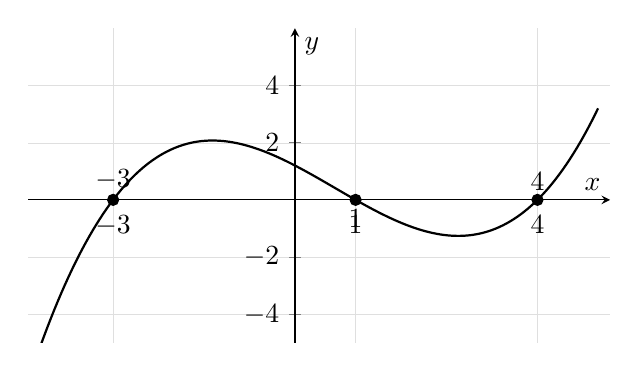
\begin{tikzpicture}
\begin{axis}[
    width=0.74\textwidth,
    height=0.46\textwidth,
    xmin=-4.4, xmax=5.2,
    ymin=-5, ymax=6,
    axis lines=middle,
    xlabel={\(x\)},
    ylabel={\(y\)},
    xtick={-3,0,1,4},
    ytick={-4,-2,0,2,4},
    grid=both,
    grid style={line width=.1pt, draw=gray!25},
]
\addplot[thick, domain=-4.2:5.0, samples=160] {0.1*(x+3)*(x-1)*(x-4)};
\addplot[only marks, mark=*] coordinates {(-3,0) (1,0) (4,0)};
\node[anchor=south] at (axis cs:-3,0) {\(-3\)};
\node[anchor=north] at (axis cs:1,0) {\(1\)};
\node[anchor=south] at (axis cs:4,0) {\(4\)};
\end{axis}
\end{tikzpicture}
\caption{Zeros divide the \(x\)-axis into intervals where the function has a fixed sign.}
\label{fig:chapter-2-review-cubic}
\end{figure}

\begin{enumerate}
\item What are the \(x\)-intercepts?

\item What is the \(y\)-intercept?

\item On which intervals is

\[
p(x)>0?
\]

\item On which intervals is

\[
p(x)<0?
\]

\item Is \(p\) even, odd, or neither? Explain.

\item What is the natural domain of \(p\)?

\item Does \(p\) appear to be one-to-one on all of \(\mathbb R\)? Explain using the horizontal line test.

\item Find a smaller interval on which \(p\) appears to be one-to-one.
\end{enumerate}

\subsection{Catalog practice: recognizing function families}
\label{subsec:catalog-practice}

Classify each model as linear, power-law, polynomial, rational, algebraic, trigonometric, exponential, or logarithmic. Then state a natural domain suggested by the context.

\begin{enumerate}
\item The cost of renting a bike is \(12\) dollars plus \(4\) dollars per hour:

\[
C(t)=12+4t.
\]

\item The area of a circle of radius \(r\) is

\[
A(r)=\pi r^2.
\]

\item A population doubles every \(6\) hours:

\[
P(t)=P_0\,2^{t/6}.
\]

\item The height of a Ferris wheel rider is

\[
H(t)=18+15\sin\left(\frac{\pi t}{20}\right).
\]

\item The average cost per item is

\[
A(x)=5+\frac{200}{x}.
\]

\item The upper half of a circle of radius \(5\) is

\[
y=\sqrt{25-x^2}.
\]

\item The time needed for an amount \(A\) to double under compound growth is described using

\[
\ln 2.
\]

\item A projectile height model is

\[
h(t)=-16t^2+80t+5.
\]
\end{enumerate}

\subsection{Counterexamples and proof practice}
\label{subsec:counterexamples-proof-practice}

\begin{enumerate}
\item Prove that for \(\varepsilon>0\),

\[
|x-a|<\varepsilon
\quad\Longleftrightarrow\quad
a-\varepsilon<x<a+\varepsilon.
\]

\item Give an example of a curve that fails the vertical line test.

\item Give an example of a function that fails the horizontal line test.

\item Give an example of a formula that simplifies algebraically but still has a missing input in its original form.

\item Give an example of a piecewise rule that does not define a function because one input receives two outputs.

\item Explain why

\[
F(x)=
\begin{cases}
1, & x<0,\\
2, & x\ge 0
\end{cases}
\]

does define a function, but

\[
G(x)=
\begin{cases}
1, & x\le 0,\\
2, & x\ge 0
\end{cases}
\]

does not.

\item Suppose \(f\) has an inverse function. Prove that if

\[
f(x_1)=f(x_2),
\]

then

\[
x_1=x_2.
\]

\item Show that the square function

\[
f(x)=x^2
\]

has no inverse function on all of \(\mathbb R\).

\item Show that the square function has inverse

\[
f^{-1}(x)=\sqrt{x}
\]

when its domain is restricted to \([0,\infty)\).

\item Optional. Prove that \(\sqrt2\) is not rational.

\item Optional. Let

\[
A=\{x\in\mathbb R:x^2<2\}.
\]

Explain why the least upper bound of \(A\) should be \(\sqrt2\).
\end{enumerate}

\subsection{Technology questions}
\label{subsec:technology-questions}

These problems are about using technology carefully. Use a graphing calculator or computer graphing tool when needed.

\begin{enumerate}
\item Graph

\[
f(x)=x^3-6x
\]

in the window

\[
-1\le x\le 1,\qquad -6\le y\le 6.
\]

Then graph it in the window

\[
-3\le x\le 3,\qquad -10\le y\le 10.
\]

What does the wider window reveal?

\item Graph

\[
h(x)=\frac{x^2-1}{x-1}
\]

and

\[
\ell(x)=x+1
\]

in the same window. What difference might the screen hide?

\item Graph

\[
f(x)=\sin(100\pi x)
\]

on

\[
0\le x\le 1.
\]

Try different sample settings if your software allows it. Explain why a poor sample can make this function look like \(0\).

\item Use a calculator to evaluate

\[
Q(h)=\frac{\sqrt{1+h}-1}{h}
\]

for

\[
h=10^{-2},\ 10^{-4},\ 10^{-8},\ 10^{-12}.
\]

Then evaluate the algebraically equivalent expression

\[
Q(h)=\frac{1}{\sqrt{1+h}+1}.
\]

Compare the results. What does this show about roundoff?

\item Find a graphing window in which

\[
g(x)=x^2+0.001\sin(1000x)
\]

looks almost like

\[
f(x)=x^2.
\]

Then zoom in until the oscillation becomes visible.

\item A graph suggests that

\[
x^2-2x+2>0
\]

for all real \(x\). Prove the claim algebraically by completing the square.
\end{enumerate}

\subsection{Project: fit a simple model to data}
\label{subsec:project-fit-simple-model}

A cup of coffee is placed in a room whose temperature is \(22^\circ\)C. The table shows measured coffee temperatures.

\[
\begin{array}{c|cccccc}
t\text{ (minutes)} & 0 & 5 & 10 & 15 & 20 & 25 \\ \hline
T(t)\text{ (degrees C)} & 90 & 73 & 60 & 51 & 44 & 39
\end{array}
\]

\begin{figure}[h]
\centering
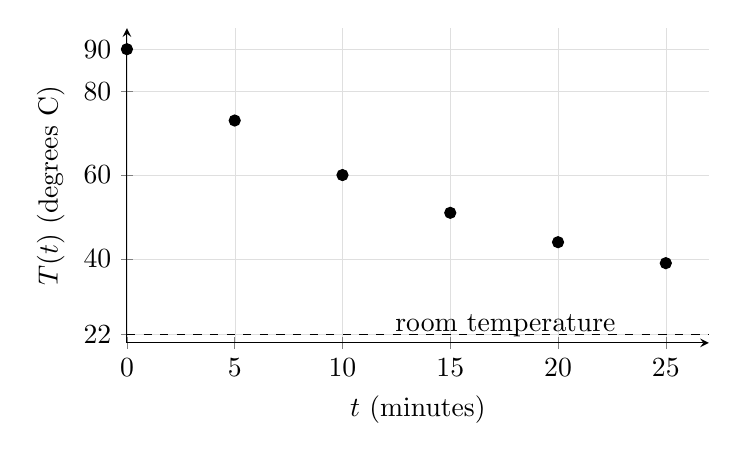
\begin{tikzpicture}
\begin{axis}[
    width=0.74\textwidth,
    height=0.46\textwidth,
    xmin=0, xmax=27,
    ymin=20, ymax=95,
    axis lines=left,
    xlabel={\(t\) (minutes)},
    ylabel={\(T(t)\) (degrees C)},
    xtick={0,5,10,15,20,25},
    ytick={22,40,60,80,90},
    grid=both,
    grid style={line width=.1pt, draw=gray!25},
]
\addplot[only marks, mark=*] coordinates {
    (0,90) (5,73) (10,60) (15,51) (20,44) (25,39)
};
\addplot[dashed, domain=0:27, samples=2] {22};
\node[anchor=west] at (axis cs:12,24) {room temperature};
\end{axis}
\end{tikzpicture}
\caption{The coffee cools toward room temperature. A good model should respect that long-term behavior.}
\label{fig:coffee-cooling-data}
\end{figure}

\begin{enumerate}
\item Explain why a linear model may be reasonable for a short time but unreasonable forever.

\item Let

\[
E(t)=T(t)-22
\]

be the excess temperature above the room. Complete the table:

\[
\begin{array}{c|cccccc}
t\text{ (minutes)} & 0 & 5 & 10 & 15 & 20 & 25 \\ \hline
E(t) & & & & & &
\end{array}
\]

\item Compute the ratios

\[
\frac{E(5)}{E(0)},\quad
\frac{E(10)}{E(5)},\quad
\frac{E(15)}{E(10)},\quad
\frac{E(20)}{E(15)},\quad
\frac{E(25)}{E(20)}.
\]

Are they roughly constant?

\item Use the first two data points to build a model of the form

\[
T(t)=22+A\,b^{t/5}.
\]

Find \(A\) and \(b\).

\item Use your model to predict the coffee temperature after \(30\) minutes.

\item Compute the residuals

\[
\text{measured temperature} - \text{predicted temperature}
\]

at the measured times.

\item Does the model overpredict, underpredict, or stay fairly balanced?

\item Explain why the horizontal line

\[
T=22
\]

should be a long-term guide for the model.

\item Optional. Compare your exponential cooling model with a linear model made from the first and last data points. Which model gives a more reasonable prediction after \(2\) hours?
\end{enumerate}

\subsection{Discovery problems}
\label{subsec:chapter-2-discovery-problems}

\begin{enumerate}
\item \textbf{Same formula, different story.}
Consider the formula

\[
y=x^2.
\]

Use four different domains:

\[
\mathbb R,\qquad [0,\infty),\qquad [-2,2],\qquad [1,3].
\]

For each domain, find the range and decide whether the function has an inverse.

\item \textbf{A hidden composition.}
Write each function as a composition of simpler functions.

\[
\sqrt{3x+1},
\qquad
(5-x^2)^4,
\qquad
\ln(1+x^2),
\qquad
\sin(2x-7).
\]

For each one, name the inside function and the outside function.

\item \textbf{How close is close?}
For

\[
Q(h)=4+h,
\]

find a condition on \(h\) that guarantees

\[
|Q(h)-4|<0.001.
\]

Then do the same for

\[
R(h)=12+6h+h^2
\]

under the extra assumption

\[
|h|<1.
\]

\item \textbf{A graph that fools the eye.}
Find two functions that look nearly identical in a wide graphing window but have different behavior when you zoom in. Explain the difference.

\item \textbf{Model choice.}
Create a table of six data points that would suggest a linear model. Then create a different table of six data points that would suggest an exponential model. Explain how the differences or ratios reveal the pattern.

\item \textbf{Rational approximations to \(\sqrt2\).}
Use a calculator to find decimal intervals of length

\[
0.1,\quad 0.01,\quad 0.001,\quad 0.0001
\]

that contain \(\sqrt2\). Write the nested intervals. What real number do they trap?

\item \textbf{Punctured intervals.}
Explain why the difference quotient

\[
\frac{f(a+h)-f(a)}{h}
\]

is naturally studied on a punctured interval around \(h=0\), rather than on an interval that includes \(h=0\).

\item \textbf{The first limit proof hiding in Chapter 1.}
For

\[
s(t)=t^2,
\]

the average velocity from \(t=2\) to \(t=2+h\) is

\[
4+h.
\]

Given an allowed error \(\varepsilon>0\), find a condition on \(h\) that guarantees

\[
|(4+h)-4|<\varepsilon.
\]

Write your answer in the form

\[
0<|h|<\delta.
\]
\end{enumerate}

\subsection{Hook: limits make near into mathematics}
\label{subsec:hook-limits-make-near}

The last problem is the doorway to the next chapter.

For

\[
s(t)=t^2,
\]

the average velocity from \(t=2\) to \(t=2+h\) is

\[
4+h,
\qquad h\neq0.
\]

As \(h\) gets close to \(0\), the average velocity gets close to \(4\). Chapter 2 gave us the language to make that sentence sharper:

\[
|(4+h)-4|=|h|.
\]

So if we want the output error to be less than \(\varepsilon\), we can demand

\[
0<|h|<\varepsilon.
\]

This is the shape of a limit. The input is allowed to approach a forbidden or special value. The output is forced into any desired error bound.

The next chapter gives this idea its name.
